\documentclass{article}

\usepackage[margin=4.00055cm,nohead,a4paper,truedimen,dvips]{geometry}
\usepackage{epic}
\usepackage{eepic}
\usepackage{lscape}
\usepackage{pgfplots}
%\pgfplotsset{compat=newest}
\usetikzlibrary{calc,decorations,decorations.pathreplacing}

\addtolength{\textheight}{-3.65\baselineskip}

\begin{document}

\pagenumbering{gobble}

\author{}
\date{}
\title{}



\newsavebox{\one}
\savebox{\one}{

\scalebox{4}{

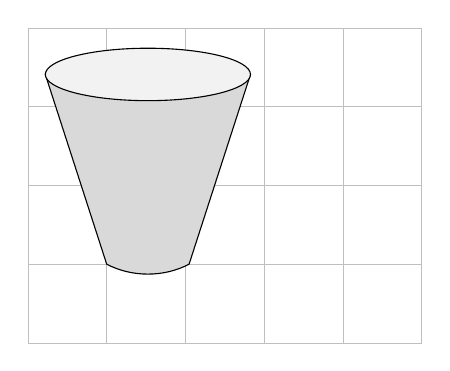
\begin{tikzpicture}

\pgfmathsetmacro{\acoor}{1.95 + random(1,3)*rnd}
\pgfmathsetmacro{\bcoor}{\acoor + rnd}
\pgfmathsetmacro{\ccoor}{.5 + .5*\acoor}
\pgfmathsetmacro{\first}{1 + (.4*\acoor - .5)}
\pgfmathsetmacro{\second}{1 + (.6*\acoor - .5)}
\pgfmathsetmacro{\split}{(2*\bcoor - 1 - \acoor)/2}
\pgfmathsetmacro{\ycoor}{1.5 + 2*rnd}
\pgfmathsetmacro{\corr}{.075 * \ycoor}
\pgfmathsetmacro{\abcorr}{(.08*(\bcoor - 1)) + .0065* \ycoor}


\draw [help lines,lightgray] (0,0) grid (5,4) ;
\draw[fill=gray!30] (1,1) .. controls (\first,1 - \abcorr) and (\second,1 - \abcorr) .. (\acoor,1) -- (\bcoor,\ycoor) --  (1 + \acoor - \bcoor,\ycoor) -- (1,1) ;
\draw[fill=gray!10] (\ccoor,\ycoor) ellipse (\split cm and \split*\corr cm) ;


\end{tikzpicture}
}

}

\newsavebox{\two}
\savebox{\two}{

\scalebox{4}{

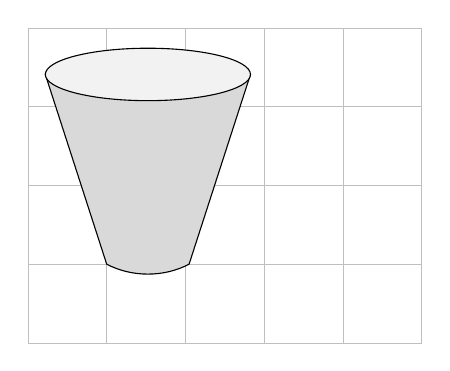
\begin{tikzpicture}

\pgfmathsetmacro{\acoor}{1.95 + random(1,3)*rnd}
\pgfmathsetmacro{\bcoor}{\acoor + rnd}
\pgfmathsetmacro{\ccoor}{.5 + .5*\acoor}
\pgfmathsetmacro{\first}{1 + (.4*\acoor - .5)}
\pgfmathsetmacro{\second}{1 + (.6*\acoor - .5)}
\pgfmathsetmacro{\split}{(2*\bcoor - 1 - \acoor)/2}
\pgfmathsetmacro{\ycoor}{1.5 + 2*rnd}
\pgfmathsetmacro{\corr}{.075 * \ycoor}
\pgfmathsetmacro{\abcorr}{(.08*(\bcoor - 1)) + .0065* \ycoor}


\draw [help lines,lightgray] (0,0) grid (5,4) ;
\draw[fill=gray!30] (1,1) .. controls (\first,1 - \abcorr) and (\second,1 - \abcorr) .. (\acoor,1) -- (\bcoor,\ycoor) --  (1 + \acoor - \bcoor,\ycoor) -- (1,1) ;
\draw[fill=gray!10] (\ccoor,\ycoor) ellipse (\split cm and \split*\corr cm) ;

\end{tikzpicture}
}

}

\newsavebox{\three}
\savebox{\three}{

\scalebox{4}{

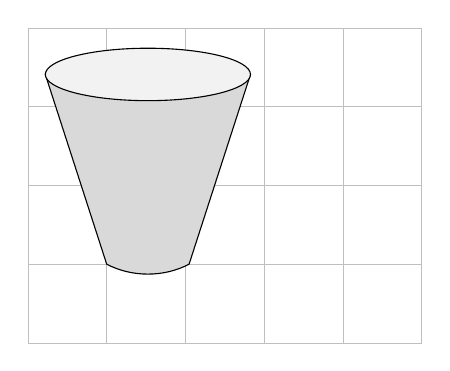
\begin{tikzpicture}

\pgfmathsetmacro{\acoor}{1.95 + random(1,3)*rnd}
\pgfmathsetmacro{\bcoor}{\acoor + rnd}
\pgfmathsetmacro{\ccoor}{.5 + .5*\acoor}
\pgfmathsetmacro{\first}{1 + (.4*\acoor - .5)}
\pgfmathsetmacro{\second}{1 + (.6*\acoor - .5)}
\pgfmathsetmacro{\split}{(2*\bcoor - 1 - \acoor)/2}
\pgfmathsetmacro{\ycoor}{1.5 + 2*rnd}
\pgfmathsetmacro{\corr}{.075 * \ycoor}
\pgfmathsetmacro{\abcorr}{(.08*(\bcoor - 1)) + .0065* \ycoor}


\draw [help lines,lightgray] (0,0) grid (5,4) ;
\draw[fill=gray!30] (1,1) .. controls (\first,1 - \abcorr) and (\second,1 - \abcorr) .. (\acoor,1) -- (\bcoor,\ycoor) --  (1 + \acoor - \bcoor,\ycoor) -- (1,1) ;
\draw[fill=gray!10] (\ccoor,\ycoor) ellipse (\split cm and \split*\corr cm) ;

\end{tikzpicture}
}

}

\newsavebox{\four}
\savebox{\four}{

\scalebox{4}{

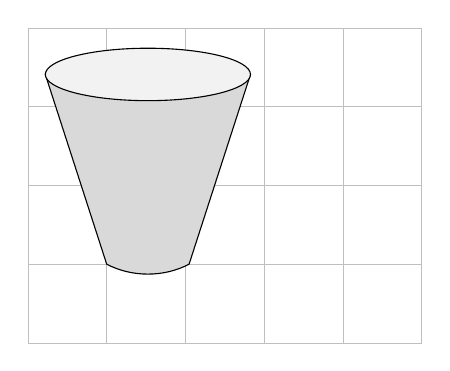
\begin{tikzpicture}

\pgfmathsetmacro{\acoor}{1.95 + random(1,3)*rnd}
\pgfmathsetmacro{\bcoor}{\acoor + rnd}
\pgfmathsetmacro{\ccoor}{.5 + .5*\acoor}
\pgfmathsetmacro{\first}{1 + (.4*\acoor - .5)}
\pgfmathsetmacro{\second}{1 + (.6*\acoor - .5)}
\pgfmathsetmacro{\split}{(2*\bcoor - 1 - \acoor)/2}
\pgfmathsetmacro{\ycoor}{1.5 + 2*rnd}
\pgfmathsetmacro{\corr}{.075 * \ycoor}
\pgfmathsetmacro{\abcorr}{(.08*(\bcoor - 1)) + .0065* \ycoor}


\draw [help lines,lightgray] (0,0) grid (5,4) ;
\draw[fill=gray!30] (1,1) .. controls (\first,1 - \abcorr) and (\second,1 - \abcorr) .. (\acoor,1) -- (\bcoor,\ycoor) --  (1 + \acoor - \bcoor,\ycoor) -- (1,1) ;
\draw[fill=gray!10] (\ccoor,\ycoor) ellipse (\split cm and \split*\corr cm) ;

\end{tikzpicture}
}

}

\newsavebox{\five}
\savebox{\five}{

\scalebox{4}{

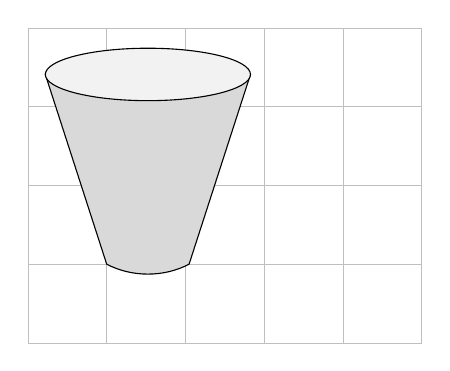
\begin{tikzpicture}

\pgfmathsetmacro{\acoor}{1.95 + random(1,3)*rnd}
\pgfmathsetmacro{\bcoor}{\acoor + rnd}
\pgfmathsetmacro{\ccoor}{.5 + .5*\acoor}
\pgfmathsetmacro{\first}{1 + (.4*\acoor - .5)}
\pgfmathsetmacro{\second}{1 + (.6*\acoor - .5)}
\pgfmathsetmacro{\split}{(2*\bcoor - 1 - \acoor)/2}
\pgfmathsetmacro{\ycoor}{1.5 + 2*rnd}
\pgfmathsetmacro{\corr}{.075 * \ycoor}
\pgfmathsetmacro{\abcorr}{(.08*(\bcoor - 1)) + .0065* \ycoor}


\draw [help lines,lightgray] (0,0) grid (5,4) ;
\draw[fill=gray!30] (1,1) .. controls (\first,1 - \abcorr) and (\second,1 - \abcorr) .. (\acoor,1) -- (\bcoor,\ycoor) --  (1 + \acoor - \bcoor,\ycoor) -- (1,1) ;
\draw[fill=gray!10] (\ccoor,\ycoor) ellipse (\split cm and \split*\corr cm) ;

\end{tikzpicture}
}

}

\newsavebox{\six}
\savebox{\six}{

\scalebox{4}{

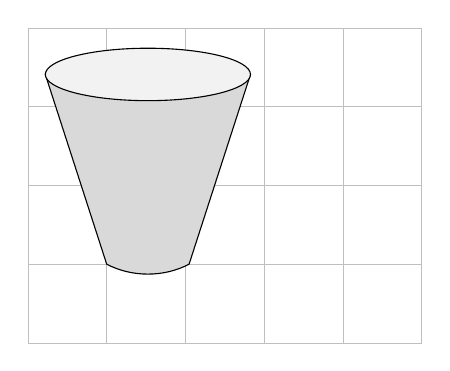
\begin{tikzpicture}

\pgfmathsetmacro{\acoor}{1.95 + random(1,3)*rnd}
\pgfmathsetmacro{\bcoor}{\acoor + rnd}
\pgfmathsetmacro{\ccoor}{.5 + .5*\acoor}
\pgfmathsetmacro{\first}{1 + (.4*\acoor - .5)}
\pgfmathsetmacro{\second}{1 + (.6*\acoor - .5)}
\pgfmathsetmacro{\split}{(2*\bcoor - 1 - \acoor)/2}
\pgfmathsetmacro{\ycoor}{1.5 + 2*rnd}
\pgfmathsetmacro{\corr}{.075 * \ycoor}
\pgfmathsetmacro{\abcorr}{(.08*(\bcoor - 1)) + .0065* \ycoor}


\draw [help lines,lightgray] (0,0) grid (5,4) ;
\draw[fill=gray!30] (1,1) .. controls (\first,1 - \abcorr) and (\second,1 - \abcorr) .. (\acoor,1) -- (\bcoor,\ycoor) --  (1 + \acoor - \bcoor,\ycoor) -- (1,1) ;
\draw[fill=gray!10] (\ccoor,\ycoor) ellipse (\split cm and \split*\corr cm) ;

\end{tikzpicture}
}

}
\newsavebox{\seven}
\savebox{\seven}{

\scalebox{4}{

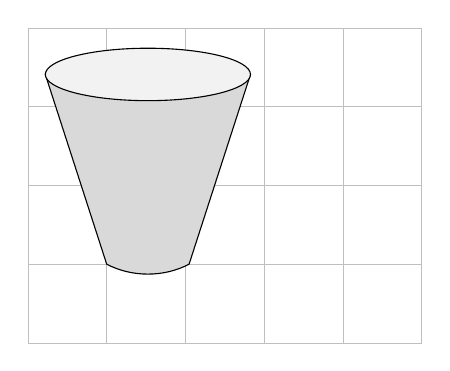
\begin{tikzpicture}

\pgfmathsetmacro{\acoor}{1.95 + random(1,3)*rnd}
\pgfmathsetmacro{\bcoor}{\acoor + rnd}
\pgfmathsetmacro{\ccoor}{.5 + .5*\acoor}
\pgfmathsetmacro{\first}{1 + (.4*\acoor - .5)}
\pgfmathsetmacro{\second}{1 + (.6*\acoor - .5)}
\pgfmathsetmacro{\split}{(2*\bcoor - 1 - \acoor)/2}
\pgfmathsetmacro{\ycoor}{1.5 + 2*rnd}
\pgfmathsetmacro{\corr}{.075 * \ycoor}
\pgfmathsetmacro{\abcorr}{(.08*(\bcoor - 1)) + .0065* \ycoor}


\draw [help lines,lightgray] (0,0) grid (5,4) ;
\draw[fill=gray!30] (1,1) .. controls (\first,1 - \abcorr) and (\second,1 - \abcorr) .. (\acoor,1) -- (\bcoor,\ycoor) --  (1 + \acoor - \bcoor,\ycoor) -- (1,1) ;
\draw[fill=gray!10] (\ccoor,\ycoor) ellipse (\split cm and \split*\corr cm) ;

\end{tikzpicture}
}

}
\newsavebox{\eight}
\savebox{\eight}{

\scalebox{4}{

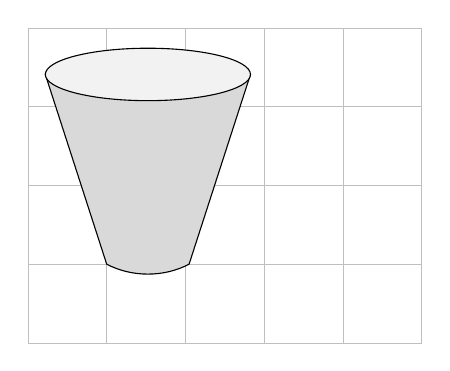
\begin{tikzpicture}

\pgfmathsetmacro{\acoor}{1.95 + random(1,3)*rnd}
\pgfmathsetmacro{\bcoor}{\acoor + rnd}
\pgfmathsetmacro{\ccoor}{.5 + .5*\acoor}
\pgfmathsetmacro{\first}{1 + (.4*\acoor - .5)}
\pgfmathsetmacro{\second}{1 + (.6*\acoor - .5)}
\pgfmathsetmacro{\split}{(2*\bcoor - 1 - \acoor)/2}
\pgfmathsetmacro{\ycoor}{1.5 + 2*rnd}
\pgfmathsetmacro{\corr}{.075 * \ycoor}
\pgfmathsetmacro{\abcorr}{(.08*(\bcoor - 1)) + .0065* \ycoor}


\draw [help lines,lightgray] (0,0) grid (5,4) ;
\draw[fill=gray!30] (1,1) .. controls (\first,1 - \abcorr) and (\second,1 - \abcorr) .. (\acoor,1) -- (\bcoor,\ycoor) --  (1 + \acoor - \bcoor,\ycoor) -- (1,1) ;
\draw[fill=gray!10] (\ccoor,\ycoor) ellipse (\split cm and \split*\corr cm) ;

\end{tikzpicture}
}

}
\newsavebox{\nine}
\savebox{\nine}{

\scalebox{4}{

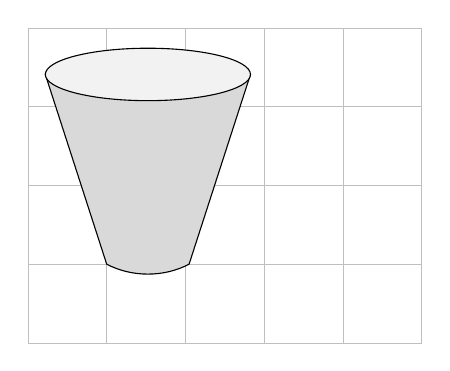
\begin{tikzpicture}

\pgfmathsetmacro{\acoor}{1.95 + random(1,3)*rnd}
\pgfmathsetmacro{\bcoor}{\acoor + rnd}
\pgfmathsetmacro{\ccoor}{.5 + .5*\acoor}
\pgfmathsetmacro{\first}{1 + (.4*\acoor - .5)}
\pgfmathsetmacro{\second}{1 + (.6*\acoor - .5)}
\pgfmathsetmacro{\split}{(2*\bcoor - 1 - \acoor)/2}
\pgfmathsetmacro{\ycoor}{1.5 + 2*rnd}
\pgfmathsetmacro{\corr}{.075 * \ycoor}
\pgfmathsetmacro{\abcorr}{(.08*(\bcoor - 1)) + .0065* \ycoor}


\draw [help lines,lightgray] (0,0) grid (5,4) ;
\draw[fill=gray!30] (1,1) .. controls (\first,1 - \abcorr) and (\second,1 - \abcorr) .. (\acoor,1) -- (\bcoor,\ycoor) --  (1 + \acoor - \bcoor,\ycoor) -- (1,1) ;
\draw[fill=gray!10] (\ccoor,\ycoor) ellipse (\split cm and \split*\corr cm) ;

\end{tikzpicture}
}

}

\newsavebox{\ten}
\savebox{\ten}{

\scalebox{4}{

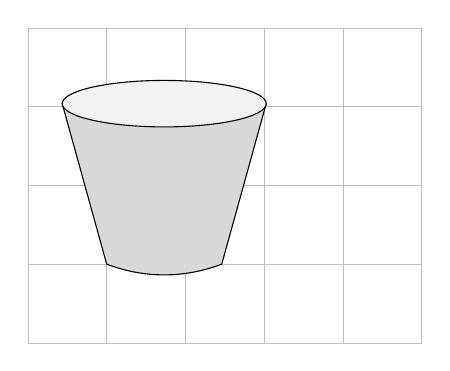
\begin{tikzpicture}

\pgfmathsetmacro{\acoor}{1.95 + random(1,3)*rnd}
\pgfmathsetmacro{\bcoor}{\acoor + rnd}
\pgfmathsetmacro{\ccoor}{.5 + .5*\acoor}
\pgfmathsetmacro{\first}{1 + (.4*\acoor - .5)}
\pgfmathsetmacro{\second}{1 + (.6*\acoor - .5)}
\pgfmathsetmacro{\split}{(2*\bcoor - 1 - \acoor)/2}
\pgfmathsetmacro{\ycoor}{1.5 + 2*rnd}
\pgfmathsetmacro{\corr}{.075 * \ycoor}
\pgfmathsetmacro{\abcorr}{(.08*(\bcoor - 1)) + .0065* \ycoor}


\draw [help lines,lightgray] (0,0) grid (5,4) ;
\draw[fill=gray!30] (1,1) .. controls (\first,1 - \abcorr) and (\second,1 - \abcorr) .. (\acoor,1) -- (\bcoor,\ycoor) --  (1 + \acoor - \bcoor,\ycoor) -- (1,1) ;
\draw[fill=gray!10] (\ccoor,\ycoor) ellipse (\split cm and \split*\corr cm) ;

\end{tikzpicture}
}

}

\newsavebox{\eleven}
\savebox{\eleven}{

\scalebox{4}{

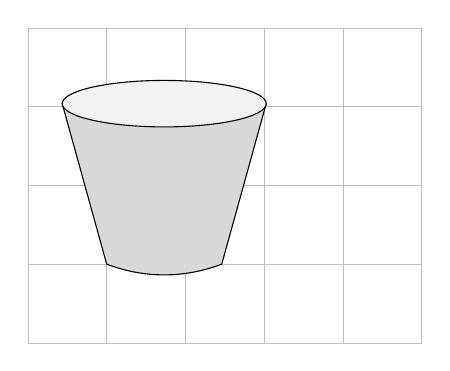
\begin{tikzpicture}

\pgfmathsetmacro{\acoor}{1.95 + random(1,3)*rnd}
\pgfmathsetmacro{\bcoor}{\acoor + rnd}
\pgfmathsetmacro{\ccoor}{.5 + .5*\acoor}
\pgfmathsetmacro{\first}{1 + (.4*\acoor - .5)}
\pgfmathsetmacro{\second}{1 + (.6*\acoor - .5)}
\pgfmathsetmacro{\split}{(2*\bcoor - 1 - \acoor)/2}
\pgfmathsetmacro{\ycoor}{1.5 + 2*rnd}
\pgfmathsetmacro{\corr}{.075 * \ycoor}
\pgfmathsetmacro{\abcorr}{(.08*(\bcoor - 1)) + .0065* \ycoor}


\draw [help lines,lightgray] (0,0) grid (5,4) ;
\draw[fill=gray!30] (1,1) .. controls (\first,1 - \abcorr) and (\second,1 - \abcorr) .. (\acoor,1) -- (\bcoor,\ycoor) --  (1 + \acoor - \bcoor,\ycoor) -- (1,1) ;
\draw[fill=gray!10] (\ccoor,\ycoor) ellipse (\split cm and \split*\corr cm) ;

\end{tikzpicture}
}

}
\newsavebox{\twelve}
\savebox{\twelve}{

\scalebox{4}{

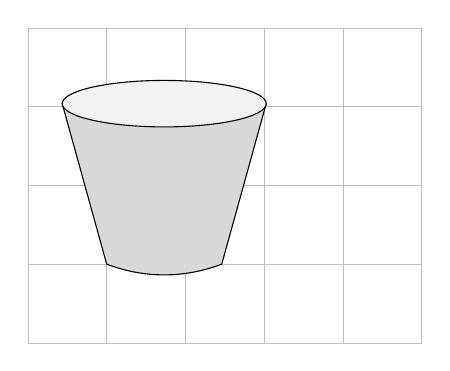
\begin{tikzpicture}

\pgfmathsetmacro{\acoor}{1.95 + random(1,3)*rnd}
\pgfmathsetmacro{\bcoor}{\acoor + rnd}
\pgfmathsetmacro{\ccoor}{.5 + .5*\acoor}
\pgfmathsetmacro{\first}{1 + (.4*\acoor - .5)}
\pgfmathsetmacro{\second}{1 + (.6*\acoor - .5)}
\pgfmathsetmacro{\split}{(2*\bcoor - 1 - \acoor)/2}
\pgfmathsetmacro{\ycoor}{1.5 + 2*rnd}
\pgfmathsetmacro{\corr}{.075 * \ycoor}
\pgfmathsetmacro{\abcorr}{(.08*(\bcoor - 1)) + .0065* \ycoor}


\draw [help lines,lightgray] (0,0) grid (5,4) ;
\draw[fill=gray!30] (1,1) .. controls (\first,1 - \abcorr) and (\second,1 - \abcorr) .. (\acoor,1) -- (\bcoor,\ycoor) --  (1 + \acoor - \bcoor,\ycoor) -- (1,1) ;
\draw[fill=gray!10] (\ccoor,\ycoor) ellipse (\split cm and \split*\corr cm) ;

\end{tikzpicture}
}

}
\newsavebox{\thirteen}
\savebox{\thirteen}{

\scalebox{4}{

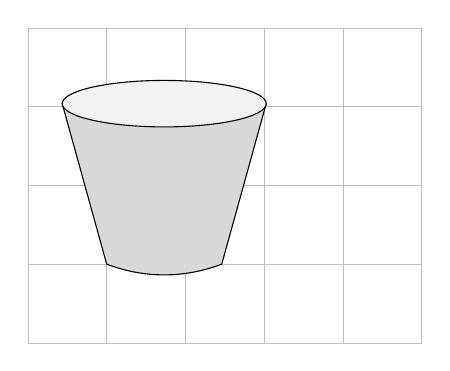
\begin{tikzpicture}

\pgfmathsetmacro{\acoor}{1.95 + random(1,3)*rnd}
\pgfmathsetmacro{\bcoor}{\acoor + rnd}
\pgfmathsetmacro{\ccoor}{.5 + .5*\acoor}
\pgfmathsetmacro{\first}{1 + (.4*\acoor - .5)}
\pgfmathsetmacro{\second}{1 + (.6*\acoor - .5)}
\pgfmathsetmacro{\split}{(2*\bcoor - 1 - \acoor)/2}
\pgfmathsetmacro{\ycoor}{1.5 + 2*rnd}
\pgfmathsetmacro{\corr}{.075 * \ycoor}
\pgfmathsetmacro{\abcorr}{(.08*(\bcoor - 1)) + .0065* \ycoor}


\draw [help lines,lightgray] (0,0) grid (5,4) ;
\draw[fill=gray!30] (1,1) .. controls (\first,1 - \abcorr) and (\second,1 - \abcorr) .. (\acoor,1) -- (\bcoor,\ycoor) --  (1 + \acoor - \bcoor,\ycoor) -- (1,1) ;
\draw[fill=gray!10] (\ccoor,\ycoor) ellipse (\split cm and \split*\corr cm) ;

\end{tikzpicture}
}

}
\newsavebox{\fourteen}
\savebox{\fourteen}{

\scalebox{4}{

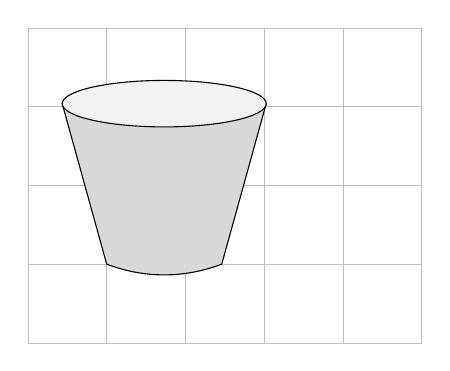
\begin{tikzpicture}

\pgfmathsetmacro{\acoor}{1.95 + random(1,3)*rnd}
\pgfmathsetmacro{\bcoor}{\acoor + rnd}
\pgfmathsetmacro{\ccoor}{.5 + .5*\acoor}
\pgfmathsetmacro{\first}{1 + (.4*\acoor - .5)}
\pgfmathsetmacro{\second}{1 + (.6*\acoor - .5)}
\pgfmathsetmacro{\split}{(2*\bcoor - 1 - \acoor)/2}
\pgfmathsetmacro{\ycoor}{1.5 + 2*rnd}
\pgfmathsetmacro{\corr}{.075 * \ycoor}
\pgfmathsetmacro{\abcorr}{(.08*(\bcoor - 1)) + .0065* \ycoor}


\draw [help lines,lightgray] (0,0) grid (5,4) ;
\draw[fill=gray!30] (1,1) .. controls (\first,1 - \abcorr) and (\second,1 - \abcorr) .. (\acoor,1) -- (\bcoor,\ycoor) --  (1 + \acoor - \bcoor,\ycoor) -- (1,1) ;
\draw[fill=gray!10] (\ccoor,\ycoor) ellipse (\split cm and \split*\corr cm) ;

\end{tikzpicture}
}

}
\newsavebox{\fifteen}
\savebox{\fifteen}{

\scalebox{4}{

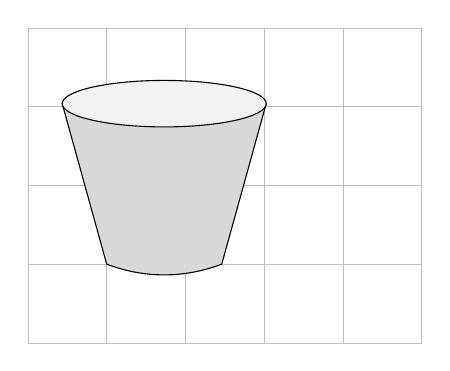
\begin{tikzpicture}

\pgfmathsetmacro{\acoor}{1.95 + random(1,3)*rnd}
\pgfmathsetmacro{\bcoor}{\acoor + rnd}
\pgfmathsetmacro{\ccoor}{.5 + .5*\acoor}
\pgfmathsetmacro{\first}{1 + (.4*\acoor - .5)}
\pgfmathsetmacro{\second}{1 + (.6*\acoor - .5)}
\pgfmathsetmacro{\split}{(2*\bcoor - 1 - \acoor)/2}
\pgfmathsetmacro{\ycoor}{1.5 + 2*rnd}
\pgfmathsetmacro{\corr}{.075 * \ycoor}
\pgfmathsetmacro{\abcorr}{(.08*(\bcoor - 1)) + .0065* \ycoor}


\draw [help lines,lightgray] (0,0) grid (5,4) ;
\draw[fill=gray!30] (1,1) .. controls (\first,1 - \abcorr) and (\second,1 - \abcorr) .. (\acoor,1) -- (\bcoor,\ycoor) --  (1 + \acoor - \bcoor,\ycoor) -- (1,1) ;
\draw[fill=gray!10] (\ccoor,\ycoor) ellipse (\split cm and \split*\corr cm) ;

\end{tikzpicture}
}

}
\newsavebox{\sixteen}
\savebox{\sixteen}{

\scalebox{4}{

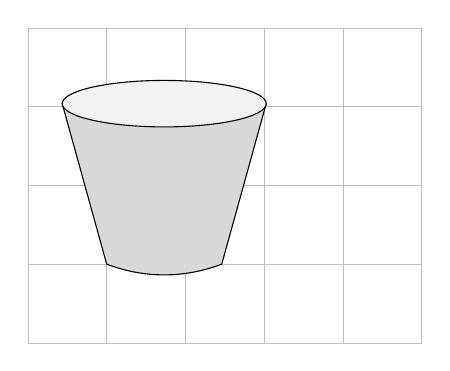
\begin{tikzpicture}

\pgfmathsetmacro{\acoor}{1.95 + random(1,3)*rnd}
\pgfmathsetmacro{\bcoor}{\acoor + rnd}
\pgfmathsetmacro{\ccoor}{.5 + .5*\acoor}
\pgfmathsetmacro{\first}{1 + (.4*\acoor - .5)}
\pgfmathsetmacro{\second}{1 + (.6*\acoor - .5)}
\pgfmathsetmacro{\split}{(2*\bcoor - 1 - \acoor)/2}
\pgfmathsetmacro{\ycoor}{1.5 + 2*rnd}
\pgfmathsetmacro{\corr}{.075 * \ycoor}
\pgfmathsetmacro{\abcorr}{(.08*(\bcoor - 1)) + .0065* \ycoor}


\draw [help lines,lightgray] (0,0) grid (5,4) ;
\draw[fill=gray!30] (1,1) .. controls (\first,1 - \abcorr) and (\second,1 - \abcorr) .. (\acoor,1) -- (\bcoor,\ycoor) --  (1 + \acoor - \bcoor,\ycoor) -- (1,1) ;
\draw[fill=gray!10] (\ccoor,\ycoor) ellipse (\split cm and \split*\corr cm) ;

\end{tikzpicture}
}

}
\newsavebox{\seventeen}
\savebox{\seventeen}{

\scalebox{4}{

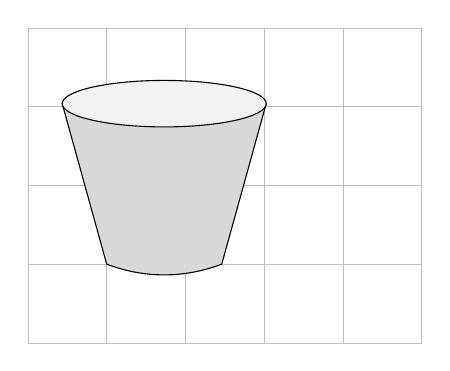
\begin{tikzpicture}

\pgfmathsetmacro{\acoor}{1.95 + random(1,3)*rnd}
\pgfmathsetmacro{\bcoor}{\acoor + rnd}
\pgfmathsetmacro{\ccoor}{.5 + .5*\acoor}
\pgfmathsetmacro{\first}{1 + (.4*\acoor - .5)}
\pgfmathsetmacro{\second}{1 + (.6*\acoor - .5)}
\pgfmathsetmacro{\split}{(2*\bcoor - 1 - \acoor)/2}
\pgfmathsetmacro{\ycoor}{1.5 + 2*rnd}
\pgfmathsetmacro{\corr}{.075 * \ycoor}
\pgfmathsetmacro{\abcorr}{(.08*(\bcoor - 1)) + .0065* \ycoor}


\draw [help lines,lightgray] (0,0) grid (5,4) ;
\draw[fill=gray!30] (1,1) .. controls (\first,1 - \abcorr) and (\second,1 - \abcorr) .. (\acoor,1) -- (\bcoor,\ycoor) --  (1 + \acoor - \bcoor,\ycoor) -- (1,1) ;
\draw[fill=gray!10] (\ccoor,\ycoor) ellipse (\split cm and \split*\corr cm) ;

\end{tikzpicture}
}

}
\newsavebox{\eightteen}
\savebox{\eightteen}{

\scalebox{4}{

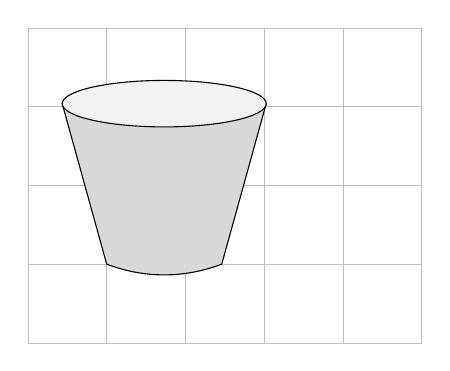
\begin{tikzpicture}

\pgfmathsetmacro{\acoor}{1.95 + random(1,3)*rnd}
\pgfmathsetmacro{\bcoor}{\acoor + rnd}
\pgfmathsetmacro{\ccoor}{.5 + .5*\acoor}
\pgfmathsetmacro{\first}{1 + (.4*\acoor - .5)}
\pgfmathsetmacro{\second}{1 + (.6*\acoor - .5)}
\pgfmathsetmacro{\split}{(2*\bcoor - 1 - \acoor)/2}
\pgfmathsetmacro{\ycoor}{1.5 + 2*rnd}
\pgfmathsetmacro{\corr}{.075 * \ycoor}
\pgfmathsetmacro{\abcorr}{(.08*(\bcoor - 1)) + .0065* \ycoor}


\draw [help lines,lightgray] (0,0) grid (5,4) ;
\draw[fill=gray!30] (1,1) .. controls (\first,1 - \abcorr) and (\second,1 - \abcorr) .. (\acoor,1) -- (\bcoor,\ycoor) --  (1 + \acoor - \bcoor,\ycoor) -- (1,1) ;
\draw[fill=gray!10] (\ccoor,\ycoor) ellipse (\split cm and \split*\corr cm) ;

\end{tikzpicture}
}

}
\newsavebox{\nineteen}
\savebox{\nineteen}{

\scalebox{4}{

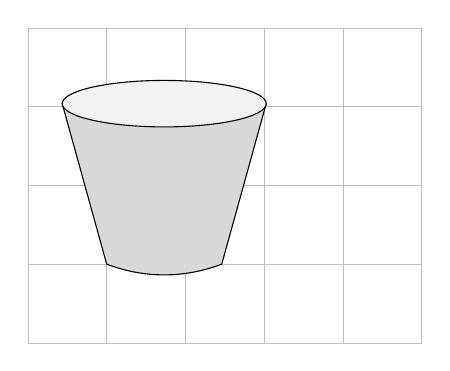
\begin{tikzpicture}

\pgfmathsetmacro{\acoor}{1.95 + random(1,3)*rnd}
\pgfmathsetmacro{\bcoor}{\acoor + rnd}
\pgfmathsetmacro{\ccoor}{.5 + .5*\acoor}
\pgfmathsetmacro{\first}{1 + (.4*\acoor - .5)}
\pgfmathsetmacro{\second}{1 + (.6*\acoor - .5)}
\pgfmathsetmacro{\split}{(2*\bcoor - 1 - \acoor)/2}
\pgfmathsetmacro{\ycoor}{1.5 + 2*rnd}
\pgfmathsetmacro{\corr}{.075 * \ycoor}
\pgfmathsetmacro{\abcorr}{(.08*(\bcoor - 1)) + .0065* \ycoor}


\draw [help lines,lightgray] (0,0) grid (5,4) ;
\draw[fill=gray!30] (1,1) .. controls (\first,1 - \abcorr) and (\second,1 - \abcorr) .. (\acoor,1) -- (\bcoor,\ycoor) --  (1 + \acoor - \bcoor,\ycoor) -- (1,1) ;
\draw[fill=gray!10] (\ccoor,\ycoor) ellipse (\split cm and \split*\corr cm) ;

\end{tikzpicture}
}

}
\newsavebox{\twenty}
\savebox{\twenty}{

\scalebox{4}{

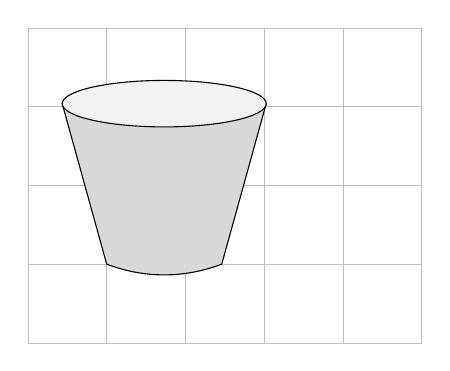
\begin{tikzpicture}

\pgfmathsetmacro{\acoor}{1.95 + random(1,3)*rnd}
\pgfmathsetmacro{\bcoor}{\acoor + rnd}
\pgfmathsetmacro{\ccoor}{.5 + .5*\acoor}
\pgfmathsetmacro{\first}{1 + (.4*\acoor - .5)}
\pgfmathsetmacro{\second}{1 + (.6*\acoor - .5)}
\pgfmathsetmacro{\split}{(2*\bcoor - 1 - \acoor)/2}
\pgfmathsetmacro{\ycoor}{1.5 + 2*rnd}
\pgfmathsetmacro{\corr}{.075 * \ycoor}
\pgfmathsetmacro{\abcorr}{(.08*(\bcoor - 1)) + .0065* \ycoor}


\draw [help lines,lightgray] (0,0) grid (5,4) ;
\draw[fill=gray!30] (1,1) .. controls (\first,1 - \abcorr) and (\second,1 - \abcorr) .. (\acoor,1) -- (\bcoor,\ycoor) --  (1 + \acoor - \bcoor,\ycoor) -- (1,1) ;
\draw[fill=gray!10] (\ccoor,\ycoor) ellipse (\split cm and \split*\corr cm) ;

\end{tikzpicture}
}

}
\newsavebox{\twentyone}
\savebox{\twentyone}{

\scalebox{4}{

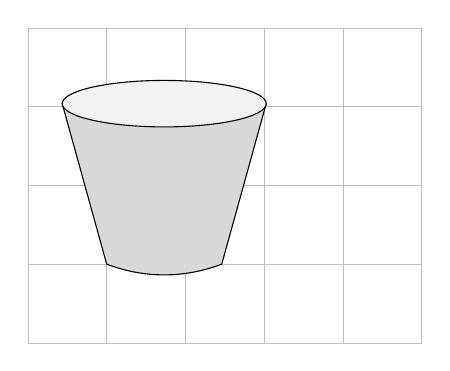
\begin{tikzpicture}

\pgfmathsetmacro{\acoor}{1.95 + random(1,3)*rnd}
\pgfmathsetmacro{\bcoor}{\acoor + rnd}
\pgfmathsetmacro{\ccoor}{.5 + .5*\acoor}
\pgfmathsetmacro{\first}{1 + (.4*\acoor - .5)}
\pgfmathsetmacro{\second}{1 + (.6*\acoor - .5)}
\pgfmathsetmacro{\split}{(2*\bcoor - 1 - \acoor)/2}
\pgfmathsetmacro{\ycoor}{1.5 + 2*rnd}
\pgfmathsetmacro{\corr}{.075 * \ycoor}
\pgfmathsetmacro{\abcorr}{(.08*(\bcoor - 1)) + .0065* \ycoor}


\draw [help lines,lightgray] (0,0) grid (5,4) ;
\draw[fill=gray!30] (1,1) .. controls (\first,1 - \abcorr) and (\second,1 - \abcorr) .. (\acoor,1) -- (\bcoor,\ycoor) --  (1 + \acoor - \bcoor,\ycoor) -- (1,1) ;
\draw[fill=gray!10] (\ccoor,\ycoor) ellipse (\split cm and \split*\corr cm) ;

\end{tikzpicture}
}

}
\newsavebox{\twentytwo}
\savebox{\twentytwo}{

\scalebox{4}{

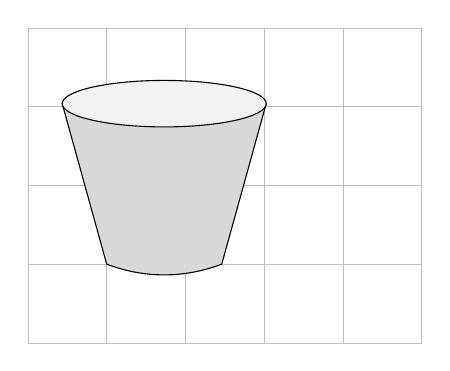
\begin{tikzpicture}

\pgfmathsetmacro{\acoor}{1.95 + random(1,3)*rnd}
\pgfmathsetmacro{\bcoor}{\acoor + rnd}
\pgfmathsetmacro{\ccoor}{.5 + .5*\acoor}
\pgfmathsetmacro{\first}{1 + (.4*\acoor - .5)}
\pgfmathsetmacro{\second}{1 + (.6*\acoor - .5)}
\pgfmathsetmacro{\split}{(2*\bcoor - 1 - \acoor)/2}
\pgfmathsetmacro{\ycoor}{1.5 + 2*rnd}
\pgfmathsetmacro{\corr}{.075 * \ycoor}
\pgfmathsetmacro{\abcorr}{(.08*(\bcoor - 1)) + .0065* \ycoor}


\draw [help lines,lightgray] (0,0) grid (5,4) ;
\draw[fill=gray!30] (1,1) .. controls (\first,1 - \abcorr) and (\second,1 - \abcorr) .. (\acoor,1) -- (\bcoor,\ycoor) --  (1 + \acoor - \bcoor,\ycoor) -- (1,1) ;
\draw[fill=gray!10] (\ccoor,\ycoor) ellipse (\split cm and \split*\corr cm) ;

\end{tikzpicture}
}

}
\newsavebox{\twentythree}
\savebox{\twentythree}{

\scalebox{4}{

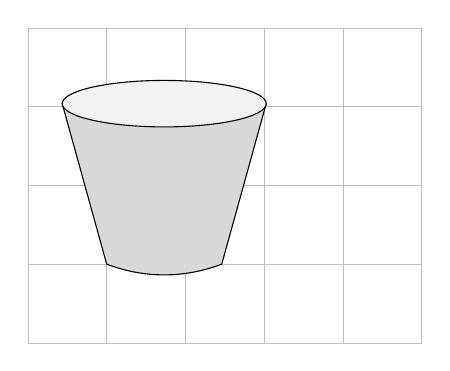
\begin{tikzpicture}

\pgfmathsetmacro{\acoor}{1.95 + random(1,3)*rnd}
\pgfmathsetmacro{\bcoor}{\acoor + rnd}
\pgfmathsetmacro{\ccoor}{.5 + .5*\acoor}
\pgfmathsetmacro{\first}{1 + (.4*\acoor - .5)}
\pgfmathsetmacro{\second}{1 + (.6*\acoor - .5)}
\pgfmathsetmacro{\split}{(2*\bcoor - 1 - \acoor)/2}
\pgfmathsetmacro{\ycoor}{1.5 + 2*rnd}
\pgfmathsetmacro{\corr}{.075 * \ycoor}
\pgfmathsetmacro{\abcorr}{(.08*(\bcoor - 1)) + .0065* \ycoor}


\draw [help lines,lightgray] (0,0) grid (5,4) ;
\draw[fill=gray!30] (1,1) .. controls (\first,1 - \abcorr) and (\second,1 - \abcorr) .. (\acoor,1) -- (\bcoor,\ycoor) --  (1 + \acoor - \bcoor,\ycoor) -- (1,1) ;
\draw[fill=gray!10] (\ccoor,\ycoor) ellipse (\split cm and \split*\corr cm) ;

\end{tikzpicture}
}

}
\newsavebox{\twentyfour}
\savebox{\twentyfour}{

\scalebox{4}{

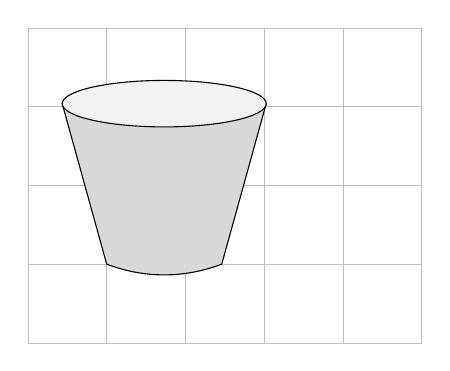
\begin{tikzpicture}

\pgfmathsetmacro{\acoor}{1.95 + random(1,3)*rnd}
\pgfmathsetmacro{\bcoor}{\acoor + rnd}
\pgfmathsetmacro{\ccoor}{.5 + .5*\acoor}
\pgfmathsetmacro{\first}{1 + (.4*\acoor - .5)}
\pgfmathsetmacro{\second}{1 + (.6*\acoor - .5)}
\pgfmathsetmacro{\split}{(2*\bcoor - 1 - \acoor)/2}
\pgfmathsetmacro{\ycoor}{1.5 + 2*rnd}
\pgfmathsetmacro{\corr}{.075 * \ycoor}
\pgfmathsetmacro{\abcorr}{(.08*(\bcoor - 1)) + .0065* \ycoor}


\draw [help lines,lightgray] (0,0) grid (5,4) ;
\draw[fill=gray!30] (1,1) .. controls (\first,1 - \abcorr) and (\second,1 - \abcorr) .. (\acoor,1) -- (\bcoor,\ycoor) --  (1 + \acoor - \bcoor,\ycoor) -- (1,1) ;
\draw[fill=gray!10] (\ccoor,\ycoor) ellipse (\split cm and \split*\corr cm) ;

\end{tikzpicture}
}

}
\newsavebox{\twentyfive}
\savebox{\twentyfive}{

\scalebox{4}{

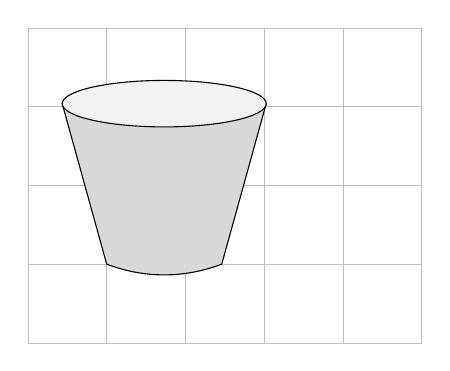
\begin{tikzpicture}

\pgfmathsetmacro{\acoor}{1.95 + random(1,3)*rnd}
\pgfmathsetmacro{\bcoor}{\acoor + rnd}
\pgfmathsetmacro{\ccoor}{.5 + .5*\acoor}
\pgfmathsetmacro{\first}{1 + (.4*\acoor - .5)}
\pgfmathsetmacro{\second}{1 + (.6*\acoor - .5)}
\pgfmathsetmacro{\split}{(2*\bcoor - 1 - \acoor)/2}
\pgfmathsetmacro{\ycoor}{1.5 + 2*rnd}
\pgfmathsetmacro{\corr}{.075 * \ycoor}
\pgfmathsetmacro{\abcorr}{(.08*(\bcoor - 1)) + .0065* \ycoor}


\draw [help lines,lightgray] (0,0) grid (5,4) ;
\draw[fill=gray!30] (1,1) .. controls (\first,1 - \abcorr) and (\second,1 - \abcorr) .. (\acoor,1) -- (\bcoor,\ycoor) --  (1 + \acoor - \bcoor,\ycoor) -- (1,1) ;
\draw[fill=gray!10] (\ccoor,\ycoor) ellipse (\split cm and \split*\corr cm) ;

\end{tikzpicture}
}

}

\newsavebox{\twentysix}
\savebox{\twentysix}{

\scalebox{4}{

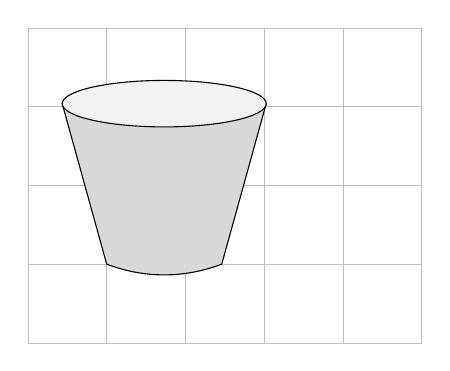
\begin{tikzpicture}

\pgfmathsetmacro{\acoor}{1.95 + random(1,3)*rnd}
\pgfmathsetmacro{\bcoor}{\acoor + rnd}
\pgfmathsetmacro{\ccoor}{.5 + .5*\acoor}
\pgfmathsetmacro{\first}{1 + (.4*\acoor - .5)}
\pgfmathsetmacro{\second}{1 + (.6*\acoor - .5)}
\pgfmathsetmacro{\split}{(2*\bcoor - 1 - \acoor)/2}
\pgfmathsetmacro{\ycoor}{1.5 + 2*rnd}
\pgfmathsetmacro{\corr}{.075 * \ycoor}
\pgfmathsetmacro{\abcorr}{(.08*(\bcoor - 1)) + .0065* \ycoor}


\draw [help lines,lightgray] (0,0) grid (5,4) ;
\draw[fill=gray!30] (1,1) .. controls (\first,1 - \abcorr) and (\second,1 - \abcorr) .. (\acoor,1) -- (\bcoor,\ycoor) --  (1 + \acoor - \bcoor,\ycoor) -- (1,1) ;
\draw[fill=gray!10] (\ccoor,\ycoor) ellipse (\split cm and \split*\corr cm) ;

\end{tikzpicture}
}

}

\newsavebox{\twentyseven}
\savebox{\twentyseven}{

\scalebox{4}{

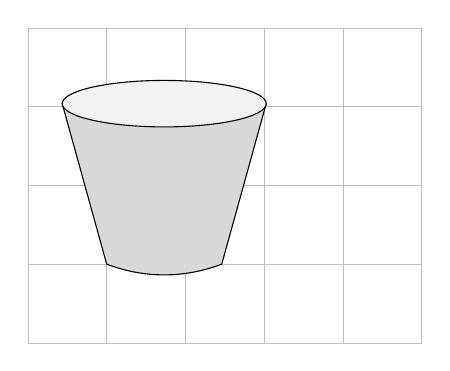
\begin{tikzpicture}

\pgfmathsetmacro{\acoor}{1.95 + random(1,3)*rnd}
\pgfmathsetmacro{\bcoor}{\acoor + rnd}
\pgfmathsetmacro{\ccoor}{.5 + .5*\acoor}
\pgfmathsetmacro{\first}{1 + (.4*\acoor - .5)}
\pgfmathsetmacro{\second}{1 + (.6*\acoor - .5)}
\pgfmathsetmacro{\split}{(2*\bcoor - 1 - \acoor)/2}
\pgfmathsetmacro{\ycoor}{1.5 + 2*rnd}
\pgfmathsetmacro{\corr}{.075 * \ycoor}
\pgfmathsetmacro{\abcorr}{(.08*(\bcoor - 1)) + .0065* \ycoor}


\draw [help lines,lightgray] (0,0) grid (5,4) ;
\draw[fill=gray!30] (1,1) .. controls (\first,1 - \abcorr) and (\second,1 - \abcorr) .. (\acoor,1) -- (\bcoor,\ycoor) --  (1 + \acoor - \bcoor,\ycoor) -- (1,1) ;
\draw[fill=gray!10] (\ccoor,\ycoor) ellipse (\split cm and \split*\corr cm) ;

\end{tikzpicture}
}

}

\newsavebox{\twentyeight}
\savebox{\twentyeight}{

\scalebox{4}{

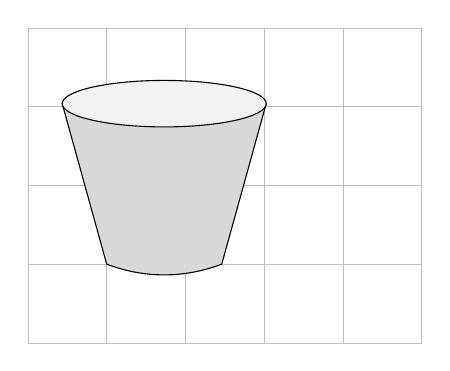
\begin{tikzpicture}

\pgfmathsetmacro{\acoor}{1.95 + random(1,3)*rnd}
\pgfmathsetmacro{\bcoor}{\acoor + rnd}
\pgfmathsetmacro{\ccoor}{.5 + .5*\acoor}
\pgfmathsetmacro{\first}{1 + (.4*\acoor - .5)}
\pgfmathsetmacro{\second}{1 + (.6*\acoor - .5)}
\pgfmathsetmacro{\split}{(2*\bcoor - 1 - \acoor)/2}
\pgfmathsetmacro{\ycoor}{1.5 + 2*rnd}
\pgfmathsetmacro{\corr}{.075 * \ycoor}
\pgfmathsetmacro{\abcorr}{(.08*(\bcoor - 1)) + .0065* \ycoor}


\draw [help lines,lightgray] (0,0) grid (5,4) ;
\draw[fill=gray!30] (1,1) .. controls (\first,1 - \abcorr) and (\second,1 - \abcorr) .. (\acoor,1) -- (\bcoor,\ycoor) --  (1 + \acoor - \bcoor,\ycoor) -- (1,1) ;
\draw[fill=gray!10] (\ccoor,\ycoor) ellipse (\split cm and \split*\corr cm) ;

\end{tikzpicture}
}

}

\newsavebox{\twentynine}
\savebox{\twentynine}{

\scalebox{4}{

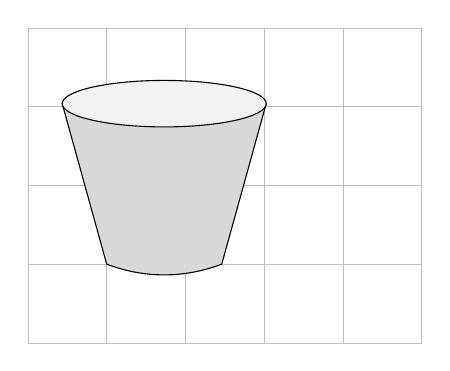
\begin{tikzpicture}

\pgfmathsetmacro{\acoor}{1.95 + random(1,3)*rnd}
\pgfmathsetmacro{\bcoor}{\acoor + rnd}
\pgfmathsetmacro{\ccoor}{.5 + .5*\acoor}
\pgfmathsetmacro{\first}{1 + (.4*\acoor - .5)}
\pgfmathsetmacro{\second}{1 + (.6*\acoor - .5)}
\pgfmathsetmacro{\split}{(2*\bcoor - 1 - \acoor)/2}
\pgfmathsetmacro{\ycoor}{1.5 + 2*rnd}
\pgfmathsetmacro{\corr}{.075 * \ycoor}
\pgfmathsetmacro{\abcorr}{(.08*(\bcoor - 1)) + .0065* \ycoor}


\draw [help lines,lightgray] (0,0) grid (5,4) ;
\draw[fill=gray!30] (1,1) .. controls (\first,1 - \abcorr) and (\second,1 - \abcorr) .. (\acoor,1) -- (\bcoor,\ycoor) --  (1 + \acoor - \bcoor,\ycoor) -- (1,1) ;
\draw[fill=gray!10] (\ccoor,\ycoor) ellipse (\split cm and \split*\corr cm) ;

\end{tikzpicture}
}

}


\newsavebox{\thirty}
\savebox{\thirty}{

\scalebox{4}{

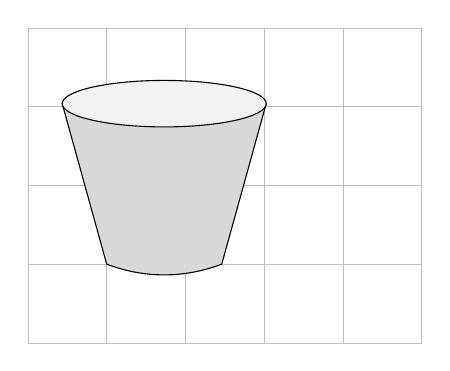
\begin{tikzpicture}

\pgfmathsetmacro{\acoor}{1.95 + random(1,3)*rnd}
\pgfmathsetmacro{\bcoor}{\acoor + rnd}
\pgfmathsetmacro{\ccoor}{.5 + .5*\acoor}
\pgfmathsetmacro{\first}{1 + (.4*\acoor - .5)}
\pgfmathsetmacro{\second}{1 + (.6*\acoor - .5)}
\pgfmathsetmacro{\split}{(2*\bcoor - 1 - \acoor)/2}
\pgfmathsetmacro{\ycoor}{1.5 + 2*rnd}
\pgfmathsetmacro{\corr}{.075 * \ycoor}
\pgfmathsetmacro{\abcorr}{(.08*(\bcoor - 1)) + .0065* \ycoor}


\draw [help lines,lightgray] (0,0) grid (5,4) ;
\draw[fill=gray!30] (1,1) .. controls (\first,1 - \abcorr) and (\second,1 - \abcorr) .. (\acoor,1) -- (\bcoor,\ycoor) --  (1 + \acoor - \bcoor,\ycoor) -- (1,1) ;
\draw[fill=gray!10] (\ccoor,\ycoor) ellipse (\split cm and \split*\corr cm) ;

\end{tikzpicture}
}

}

\newsavebox{\thirtyone}
\savebox{\thirtyone}{

\scalebox{4}{

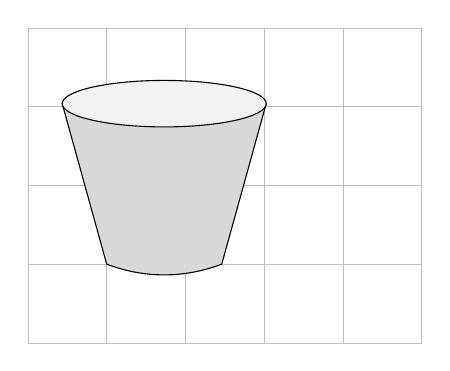
\begin{tikzpicture}

\pgfmathsetmacro{\acoor}{1.95 + random(1,3)*rnd}
\pgfmathsetmacro{\bcoor}{\acoor + rnd}
\pgfmathsetmacro{\ccoor}{.5 + .5*\acoor}
\pgfmathsetmacro{\first}{1 + (.4*\acoor - .5)}
\pgfmathsetmacro{\second}{1 + (.6*\acoor - .5)}
\pgfmathsetmacro{\split}{(2*\bcoor - 1 - \acoor)/2}
\pgfmathsetmacro{\ycoor}{1.5 + 2*rnd}
\pgfmathsetmacro{\corr}{.075 * \ycoor}
\pgfmathsetmacro{\abcorr}{(.08*(\bcoor - 1)) + .0065* \ycoor}


\draw [help lines,lightgray] (0,0) grid (5,4) ;
\draw[fill=gray!30] (1,1) .. controls (\first,1 - \abcorr) and (\second,1 - \abcorr) .. (\acoor,1) -- (\bcoor,\ycoor) --  (1 + \acoor - \bcoor,\ycoor) -- (1,1) ;
\draw[fill=gray!10] (\ccoor,\ycoor) ellipse (\split cm and \split*\corr cm) ;

\end{tikzpicture}
}

}

\newsavebox{\thirtytwo}
\savebox{\thirtytwo}{

\scalebox{4}{

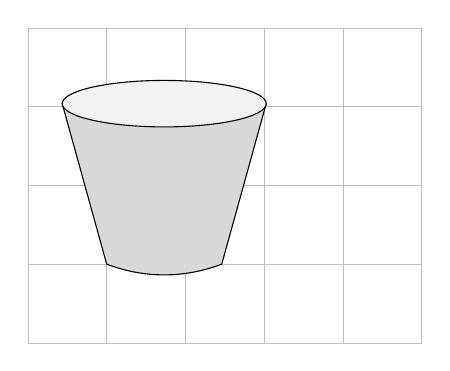
\begin{tikzpicture}

\pgfmathsetmacro{\acoor}{1.95 + random(1,3)*rnd}
\pgfmathsetmacro{\bcoor}{\acoor + rnd}
\pgfmathsetmacro{\ccoor}{.5 + .5*\acoor}
\pgfmathsetmacro{\first}{1 + (.4*\acoor - .5)}
\pgfmathsetmacro{\second}{1 + (.6*\acoor - .5)}
\pgfmathsetmacro{\split}{(2*\bcoor - 1 - \acoor)/2}
\pgfmathsetmacro{\ycoor}{1.5 + 2*rnd}
\pgfmathsetmacro{\corr}{.075 * \ycoor}
\pgfmathsetmacro{\abcorr}{(.08*(\bcoor - 1)) + .0065* \ycoor}


\draw [help lines,lightgray] (0,0) grid (5,4) ;
\draw[fill=gray!30] (1,1) .. controls (\first,1 - \abcorr) and (\second,1 - \abcorr) .. (\acoor,1) -- (\bcoor,\ycoor) --  (1 + \acoor - \bcoor,\ycoor) -- (1,1) ;
\draw[fill=gray!10] (\ccoor,\ycoor) ellipse (\split cm and \split*\corr cm) ;

\end{tikzpicture}
}

}

\newsavebox{\thirtythree}
\savebox{\thirtythree}{

\scalebox{4}{

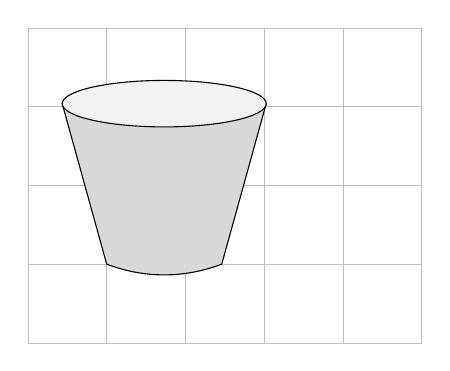
\begin{tikzpicture}

\pgfmathsetmacro{\acoor}{1.95 + random(1,3)*rnd}
\pgfmathsetmacro{\bcoor}{\acoor + rnd}
\pgfmathsetmacro{\ccoor}{.5 + .5*\acoor}
\pgfmathsetmacro{\first}{1 + (.4*\acoor - .5)}
\pgfmathsetmacro{\second}{1 + (.6*\acoor - .5)}
\pgfmathsetmacro{\split}{(2*\bcoor - 1 - \acoor)/2}
\pgfmathsetmacro{\ycoor}{1.5 + 2*rnd}
\pgfmathsetmacro{\corr}{.075 * \ycoor}
\pgfmathsetmacro{\abcorr}{(.08*(\bcoor - 1)) + .0065* \ycoor}


\draw [help lines,lightgray] (0,0) grid (5,4) ;
\draw[fill=gray!30] (1,1) .. controls (\first,1 - \abcorr) and (\second,1 - \abcorr) .. (\acoor,1) -- (\bcoor,\ycoor) --  (1 + \acoor - \bcoor,\ycoor) -- (1,1) ;
\draw[fill=gray!10] (\ccoor,\ycoor) ellipse (\split cm and \split*\corr cm) ;

\end{tikzpicture}
}

}

\newsavebox{\thirtyfour}
\savebox{\thirtyfour}{

\scalebox{4}{

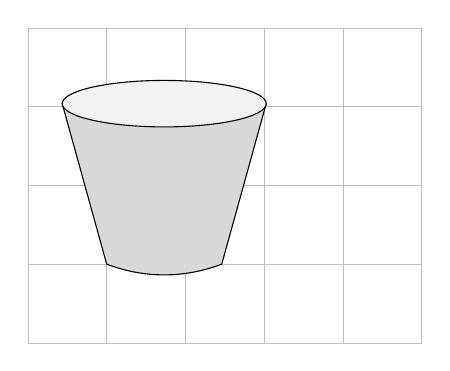
\begin{tikzpicture}

\pgfmathsetmacro{\acoor}{1.95 + random(1,3)*rnd}
\pgfmathsetmacro{\bcoor}{\acoor + rnd}
\pgfmathsetmacro{\ccoor}{.5 + .5*\acoor}
\pgfmathsetmacro{\first}{1 + (.4*\acoor - .5)}
\pgfmathsetmacro{\second}{1 + (.6*\acoor - .5)}
\pgfmathsetmacro{\split}{(2*\bcoor - 1 - \acoor)/2}
\pgfmathsetmacro{\ycoor}{1.5 + 2*rnd}
\pgfmathsetmacro{\corr}{.075 * \ycoor}
\pgfmathsetmacro{\abcorr}{(.08*(\bcoor - 1)) + .0065* \ycoor}


\draw [help lines,lightgray] (0,0) grid (5,4) ;
\draw[fill=gray!30] (1,1) .. controls (\first,1 - \abcorr) and (\second,1 - \abcorr) .. (\acoor,1) -- (\bcoor,\ycoor) --  (1 + \acoor - \bcoor,\ycoor) -- (1,1) ;
\draw[fill=gray!10] (\ccoor,\ycoor) ellipse (\split cm and \split*\corr cm) ;

\end{tikzpicture}
}

}

\newsavebox{\thirtyfive}
\savebox{\thirtyfive}{

\scalebox{4}{

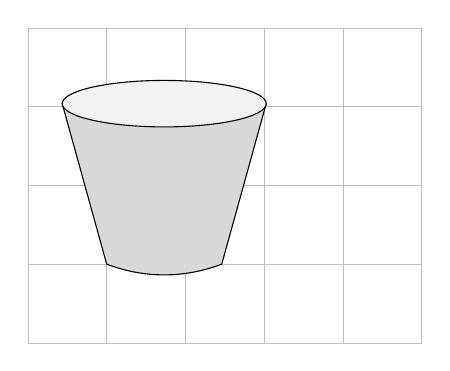
\begin{tikzpicture}

\pgfmathsetmacro{\acoor}{1.95 + random(1,3)*rnd}
\pgfmathsetmacro{\bcoor}{\acoor + rnd}
\pgfmathsetmacro{\ccoor}{.5 + .5*\acoor}
\pgfmathsetmacro{\first}{1 + (.4*\acoor - .5)}
\pgfmathsetmacro{\second}{1 + (.6*\acoor - .5)}
\pgfmathsetmacro{\split}{(2*\bcoor - 1 - \acoor)/2}
\pgfmathsetmacro{\ycoor}{1.5 + 2*rnd}
\pgfmathsetmacro{\corr}{.075 * \ycoor}
\pgfmathsetmacro{\abcorr}{(.08*(\bcoor - 1)) + .0065* \ycoor}


\draw [help lines,lightgray] (0,0) grid (5,4) ;
\draw[fill=gray!30] (1,1) .. controls (\first,1 - \abcorr) and (\second,1 - \abcorr) .. (\acoor,1) -- (\bcoor,\ycoor) --  (1 + \acoor - \bcoor,\ycoor) -- (1,1) ;
\draw[fill=gray!10] (\ccoor,\ycoor) ellipse (\split cm and \split*\corr cm) ;

\end{tikzpicture}
}

}

\newsavebox{\thirtysix}
\savebox{\thirtysix}{

\scalebox{4}{

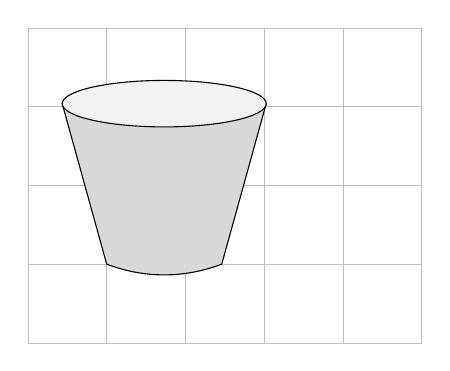
\begin{tikzpicture}

\pgfmathsetmacro{\acoor}{1.95 + random(1,3)*rnd}
\pgfmathsetmacro{\bcoor}{\acoor + rnd}
\pgfmathsetmacro{\ccoor}{.5 + .5*\acoor}
\pgfmathsetmacro{\first}{1 + (.4*\acoor - .5)}
\pgfmathsetmacro{\second}{1 + (.6*\acoor - .5)}
\pgfmathsetmacro{\split}{(2*\bcoor - 1 - \acoor)/2}
\pgfmathsetmacro{\ycoor}{1.5 + 2*rnd}
\pgfmathsetmacro{\corr}{.075 * \ycoor}
\pgfmathsetmacro{\abcorr}{(.08*(\bcoor - 1)) + .0065* \ycoor}


\draw [help lines,lightgray] (0,0) grid (5,4) ;
\draw[fill=gray!30] (1,1) .. controls (\first,1 - \abcorr) and (\second,1 - \abcorr) .. (\acoor,1) -- (\bcoor,\ycoor) --  (1 + \acoor - \bcoor,\ycoor) -- (1,1) ;
\draw[fill=gray!10] (\ccoor,\ycoor) ellipse (\split cm and \split*\corr cm) ;

\end{tikzpicture}
}

}

\newsavebox{\thirtyseven}
\savebox{\thirtyseven}{

\scalebox{4}{

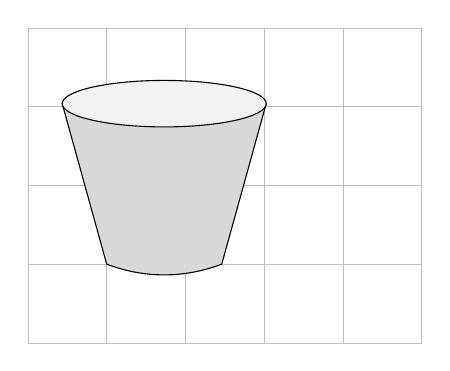
\begin{tikzpicture}

\pgfmathsetmacro{\acoor}{1.95 + random(1,3)*rnd}
\pgfmathsetmacro{\bcoor}{\acoor + rnd}
\pgfmathsetmacro{\ccoor}{.5 + .5*\acoor}
\pgfmathsetmacro{\first}{1 + (.4*\acoor - .5)}
\pgfmathsetmacro{\second}{1 + (.6*\acoor - .5)}
\pgfmathsetmacro{\split}{(2*\bcoor - 1 - \acoor)/2}
\pgfmathsetmacro{\ycoor}{1.5 + 2*rnd}
\pgfmathsetmacro{\corr}{.075 * \ycoor}
\pgfmathsetmacro{\abcorr}{(.08*(\bcoor - 1)) + .0065* \ycoor}


\draw [help lines,lightgray] (0,0) grid (5,4) ;
\draw[fill=gray!30] (1,1) .. controls (\first,1 - \abcorr) and (\second,1 - \abcorr) .. (\acoor,1) -- (\bcoor,\ycoor) --  (1 + \acoor - \bcoor,\ycoor) -- (1,1) ;
\draw[fill=gray!10] (\ccoor,\ycoor) ellipse (\split cm and \split*\corr cm) ;

\end{tikzpicture}
}

}

\newsavebox{\thirtyeight}
\savebox{\thirtyeight}{

\scalebox{4}{

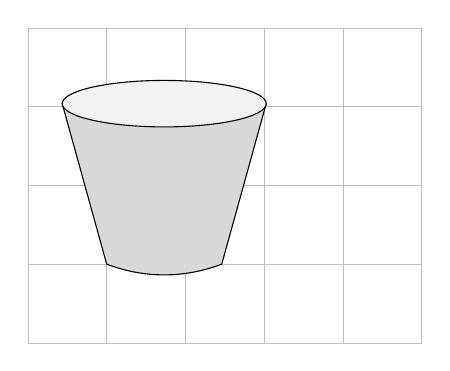
\begin{tikzpicture}

\pgfmathsetmacro{\acoor}{1.95 + random(1,3)*rnd}
\pgfmathsetmacro{\bcoor}{\acoor + rnd}
\pgfmathsetmacro{\ccoor}{.5 + .5*\acoor}
\pgfmathsetmacro{\first}{1 + (.4*\acoor - .5)}
\pgfmathsetmacro{\second}{1 + (.6*\acoor - .5)}
\pgfmathsetmacro{\split}{(2*\bcoor - 1 - \acoor)/2}
\pgfmathsetmacro{\ycoor}{1.5 + 2*rnd}
\pgfmathsetmacro{\corr}{.075 * \ycoor}
\pgfmathsetmacro{\abcorr}{(.08*(\bcoor - 1)) + .0065* \ycoor}


\draw [help lines,lightgray] (0,0) grid (5,4) ;
\draw[fill=gray!30] (1,1) .. controls (\first,1 - \abcorr) and (\second,1 - \abcorr) .. (\acoor,1) -- (\bcoor,\ycoor) --  (1 + \acoor - \bcoor,\ycoor) -- (1,1) ;
\draw[fill=gray!10] (\ccoor,\ycoor) ellipse (\split cm and \split*\corr cm) ;

\end{tikzpicture}
}

}

\newsavebox{\thirtynine}
\savebox{\thirtynine}{

\scalebox{4}{

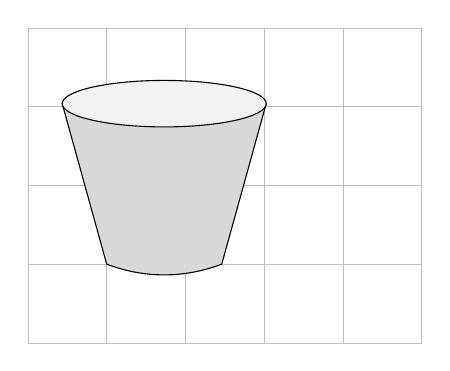
\begin{tikzpicture}

\pgfmathsetmacro{\acoor}{1.95 + random(1,3)*rnd}
\pgfmathsetmacro{\bcoor}{\acoor + rnd}
\pgfmathsetmacro{\ccoor}{.5 + .5*\acoor}
\pgfmathsetmacro{\first}{1 + (.4*\acoor - .5)}
\pgfmathsetmacro{\second}{1 + (.6*\acoor - .5)}
\pgfmathsetmacro{\split}{(2*\bcoor - 1 - \acoor)/2}
\pgfmathsetmacro{\ycoor}{1.5 + 2*rnd}
\pgfmathsetmacro{\corr}{.075 * \ycoor}
\pgfmathsetmacro{\abcorr}{(.08*(\bcoor - 1)) + .0065* \ycoor}


\draw [help lines,lightgray] (0,0) grid (5,4) ;
\draw[fill=gray!30] (1,1) .. controls (\first,1 - \abcorr) and (\second,1 - \abcorr) .. (\acoor,1) -- (\bcoor,\ycoor) --  (1 + \acoor - \bcoor,\ycoor) -- (1,1) ;
\draw[fill=gray!10] (\ccoor,\ycoor) ellipse (\split cm and \split*\corr cm) ;

\end{tikzpicture}
}

}





\newsavebox{\forty}
\savebox{\forty}{

\scalebox{4}{

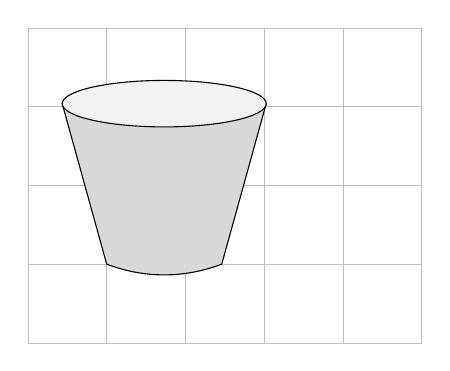
\begin{tikzpicture}

\pgfmathsetmacro{\acoor}{1.95 + random(1,3)*rnd}
\pgfmathsetmacro{\bcoor}{\acoor + rnd}
\pgfmathsetmacro{\ccoor}{.5 + .5*\acoor}
\pgfmathsetmacro{\first}{1 + (.4*\acoor - .5)}
\pgfmathsetmacro{\second}{1 + (.6*\acoor - .5)}
\pgfmathsetmacro{\split}{(2*\bcoor - 1 - \acoor)/2}
\pgfmathsetmacro{\ycoor}{1.5 + 2*rnd}
\pgfmathsetmacro{\corr}{.075 * \ycoor}
\pgfmathsetmacro{\abcorr}{(.08*(\bcoor - 1)) + .0065* \ycoor}


\draw [help lines,lightgray] (0,0) grid (5,4) ;
\draw[fill=gray!30] (1,1) .. controls (\first,1 - \abcorr) and (\second,1 - \abcorr) .. (\acoor,1) -- (\bcoor,\ycoor) --  (1 + \acoor - \bcoor,\ycoor) -- (1,1) ;
\draw[fill=gray!10] (\ccoor,\ycoor) ellipse (\split cm and \split*\corr cm) ;

\end{tikzpicture}
}

}

\newsavebox{\fortyone}
\savebox{\fortyone}{

\scalebox{4}{

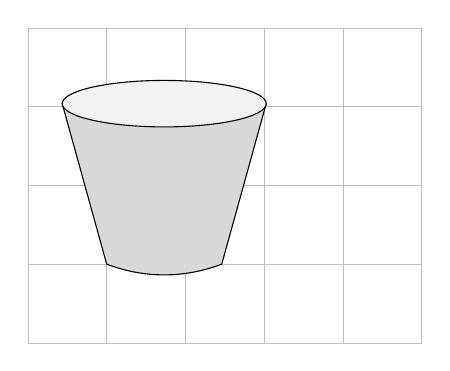
\begin{tikzpicture}

\pgfmathsetmacro{\acoor}{1.95 + random(1,3)*rnd}
\pgfmathsetmacro{\bcoor}{\acoor + rnd}
\pgfmathsetmacro{\ccoor}{.5 + .5*\acoor}
\pgfmathsetmacro{\first}{1 + (.4*\acoor - .5)}
\pgfmathsetmacro{\second}{1 + (.6*\acoor - .5)}
\pgfmathsetmacro{\split}{(2*\bcoor - 1 - \acoor)/2}
\pgfmathsetmacro{\ycoor}{1.5 + 2*rnd}
\pgfmathsetmacro{\corr}{.075 * \ycoor}
\pgfmathsetmacro{\abcorr}{(.08*(\bcoor - 1)) + .0065* \ycoor}


\draw [help lines,lightgray] (0,0) grid (5,4) ;
\draw[fill=gray!30] (1,1) .. controls (\first,1 - \abcorr) and (\second,1 - \abcorr) .. (\acoor,1) -- (\bcoor,\ycoor) --  (1 + \acoor - \bcoor,\ycoor) -- (1,1) ;
\draw[fill=gray!10] (\ccoor,\ycoor) ellipse (\split cm and \split*\corr cm) ;

\end{tikzpicture}
}

}

\newsavebox{\fortytwo}
\savebox{\fortytwo}{

\scalebox{4}{

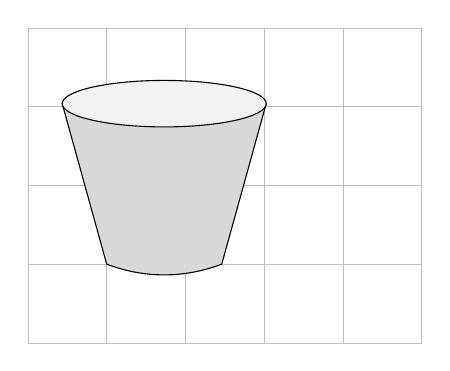
\begin{tikzpicture}

\pgfmathsetmacro{\acoor}{1.95 + random(1,3)*rnd}
\pgfmathsetmacro{\bcoor}{\acoor + rnd}
\pgfmathsetmacro{\ccoor}{.5 + .5*\acoor}
\pgfmathsetmacro{\first}{1 + (.4*\acoor - .5)}
\pgfmathsetmacro{\second}{1 + (.6*\acoor - .5)}
\pgfmathsetmacro{\split}{(2*\bcoor - 1 - \acoor)/2}
\pgfmathsetmacro{\ycoor}{1.5 + 2*rnd}
\pgfmathsetmacro{\corr}{.075 * \ycoor}
\pgfmathsetmacro{\abcorr}{(.08*(\bcoor - 1)) + .0065* \ycoor}


\draw [help lines,lightgray] (0,0) grid (5,4) ;
\draw[fill=gray!30] (1,1) .. controls (\first,1 - \abcorr) and (\second,1 - \abcorr) .. (\acoor,1) -- (\bcoor,\ycoor) --  (1 + \acoor - \bcoor,\ycoor) -- (1,1) ;
\draw[fill=gray!10] (\ccoor,\ycoor) ellipse (\split cm and \split*\corr cm) ;

\end{tikzpicture}
}

}

\newsavebox{\fortythree}
\savebox{\fortythree}{

\scalebox{4}{

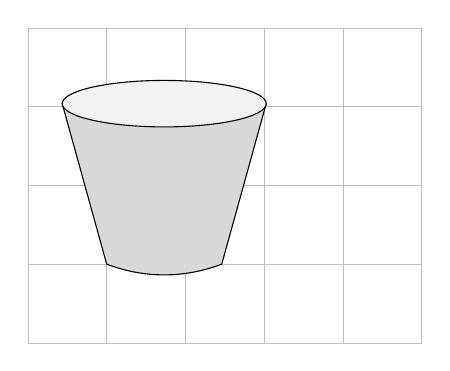
\begin{tikzpicture}

\pgfmathsetmacro{\acoor}{1.95 + random(1,3)*rnd}
\pgfmathsetmacro{\bcoor}{\acoor + rnd}
\pgfmathsetmacro{\ccoor}{.5 + .5*\acoor}
\pgfmathsetmacro{\first}{1 + (.4*\acoor - .5)}
\pgfmathsetmacro{\second}{1 + (.6*\acoor - .5)}
\pgfmathsetmacro{\split}{(2*\bcoor - 1 - \acoor)/2}
\pgfmathsetmacro{\ycoor}{1.5 + 2*rnd}
\pgfmathsetmacro{\corr}{.075 * \ycoor}
\pgfmathsetmacro{\abcorr}{(.08*(\bcoor - 1)) + .0065* \ycoor}


\draw [help lines,lightgray] (0,0) grid (5,4) ;
\draw[fill=gray!30] (1,1) .. controls (\first,1 - \abcorr) and (\second,1 - \abcorr) .. (\acoor,1) -- (\bcoor,\ycoor) --  (1 + \acoor - \bcoor,\ycoor) -- (1,1) ;
\draw[fill=gray!10] (\ccoor,\ycoor) ellipse (\split cm and \split*\corr cm) ;

\end{tikzpicture}
}

}

\newsavebox{\fortyfour}
\savebox{\fortyfour}{

\scalebox{4}{

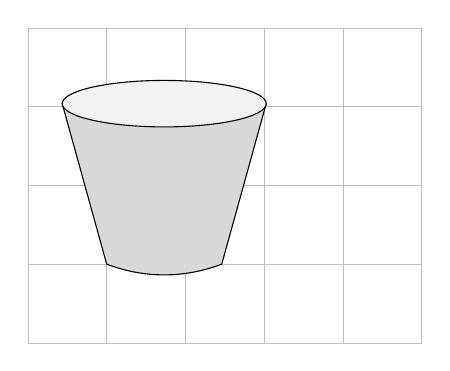
\begin{tikzpicture}

\pgfmathsetmacro{\acoor}{1.95 + random(1,3)*rnd}
\pgfmathsetmacro{\bcoor}{\acoor + rnd}
\pgfmathsetmacro{\ccoor}{.5 + .5*\acoor}
\pgfmathsetmacro{\first}{1 + (.4*\acoor - .5)}
\pgfmathsetmacro{\second}{1 + (.6*\acoor - .5)}
\pgfmathsetmacro{\split}{(2*\bcoor - 1 - \acoor)/2}
\pgfmathsetmacro{\ycoor}{1.5 + 2*rnd}
\pgfmathsetmacro{\corr}{.075 * \ycoor}
\pgfmathsetmacro{\abcorr}{(.08*(\bcoor - 1)) + .0065* \ycoor}


\draw [help lines,lightgray] (0,0) grid (5,4) ;
\draw[fill=gray!30] (1,1) .. controls (\first,1 - \abcorr) and (\second,1 - \abcorr) .. (\acoor,1) -- (\bcoor,\ycoor) --  (1 + \acoor - \bcoor,\ycoor) -- (1,1) ;
\draw[fill=gray!10] (\ccoor,\ycoor) ellipse (\split cm and \split*\corr cm) ;

\end{tikzpicture}
}

}

\newsavebox{\fortyfive}
\savebox{\fortyfive}{

\scalebox{4}{

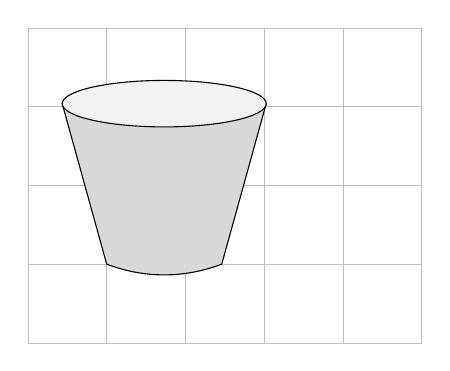
\begin{tikzpicture}

\pgfmathsetmacro{\acoor}{1.95 + random(1,3)*rnd}
\pgfmathsetmacro{\bcoor}{\acoor + rnd}
\pgfmathsetmacro{\ccoor}{.5 + .5*\acoor}
\pgfmathsetmacro{\first}{1 + (.4*\acoor - .5)}
\pgfmathsetmacro{\second}{1 + (.6*\acoor - .5)}
\pgfmathsetmacro{\split}{(2*\bcoor - 1 - \acoor)/2}
\pgfmathsetmacro{\ycoor}{1.5 + 2*rnd}
\pgfmathsetmacro{\corr}{.075 * \ycoor}
\pgfmathsetmacro{\abcorr}{(.08*(\bcoor - 1)) + .0065* \ycoor}


\draw [help lines,lightgray] (0,0) grid (5,4) ;
\draw[fill=gray!30] (1,1) .. controls (\first,1 - \abcorr) and (\second,1 - \abcorr) .. (\acoor,1) -- (\bcoor,\ycoor) --  (1 + \acoor - \bcoor,\ycoor) -- (1,1) ;
\draw[fill=gray!10] (\ccoor,\ycoor) ellipse (\split cm and \split*\corr cm) ;

\end{tikzpicture}
}

}

\newsavebox{\fortysix}
\savebox{\fortysix}{

\scalebox{4}{

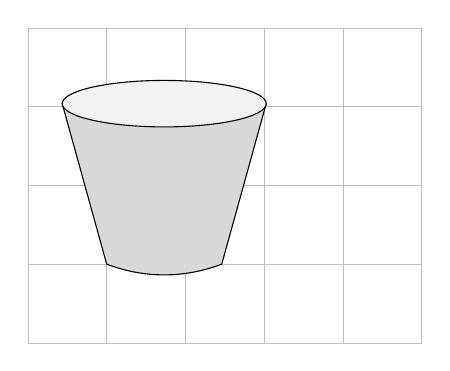
\begin{tikzpicture}

\pgfmathsetmacro{\acoor}{1.95 + random(1,3)*rnd}
\pgfmathsetmacro{\bcoor}{\acoor + rnd}
\pgfmathsetmacro{\ccoor}{.5 + .5*\acoor}
\pgfmathsetmacro{\first}{1 + (.4*\acoor - .5)}
\pgfmathsetmacro{\second}{1 + (.6*\acoor - .5)}
\pgfmathsetmacro{\split}{(2*\bcoor - 1 - \acoor)/2}
\pgfmathsetmacro{\ycoor}{1.5 + 2*rnd}
\pgfmathsetmacro{\corr}{.075 * \ycoor}
\pgfmathsetmacro{\abcorr}{(.08*(\bcoor - 1)) + .0065* \ycoor}


\draw [help lines,lightgray] (0,0) grid (5,4) ;
\draw[fill=gray!30] (1,1) .. controls (\first,1 - \abcorr) and (\second,1 - \abcorr) .. (\acoor,1) -- (\bcoor,\ycoor) --  (1 + \acoor - \bcoor,\ycoor) -- (1,1) ;
\draw[fill=gray!10] (\ccoor,\ycoor) ellipse (\split cm and \split*\corr cm) ;

\end{tikzpicture}
}

}

\newsavebox{\fortyseven}
\savebox{\fortyseven}{

\scalebox{4}{

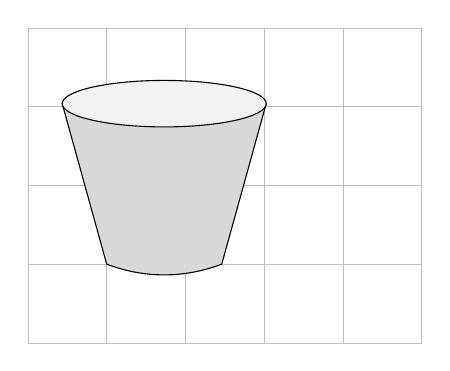
\begin{tikzpicture}

\pgfmathsetmacro{\acoor}{1.95 + random(1,3)*rnd}
\pgfmathsetmacro{\bcoor}{\acoor + rnd}
\pgfmathsetmacro{\ccoor}{.5 + .5*\acoor}
\pgfmathsetmacro{\first}{1 + (.4*\acoor - .5)}
\pgfmathsetmacro{\second}{1 + (.6*\acoor - .5)}
\pgfmathsetmacro{\split}{(2*\bcoor - 1 - \acoor)/2}
\pgfmathsetmacro{\ycoor}{1.5 + 2*rnd}
\pgfmathsetmacro{\corr}{.075 * \ycoor}
\pgfmathsetmacro{\abcorr}{(.08*(\bcoor - 1)) + .0065* \ycoor}


\draw [help lines,lightgray] (0,0) grid (5,4) ;
\draw[fill=gray!30] (1,1) .. controls (\first,1 - \abcorr) and (\second,1 - \abcorr) .. (\acoor,1) -- (\bcoor,\ycoor) --  (1 + \acoor - \bcoor,\ycoor) -- (1,1) ;
\draw[fill=gray!10] (\ccoor,\ycoor) ellipse (\split cm and \split*\corr cm) ;

\end{tikzpicture}
}

}

\newsavebox{\fortyeight}
\savebox{\fortyeight}{

\scalebox{4}{

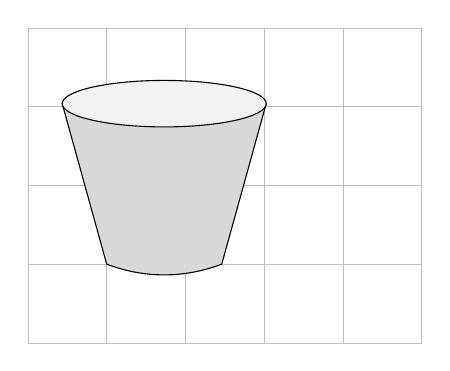
\begin{tikzpicture}

\pgfmathsetmacro{\acoor}{1.95 + random(1,3)*rnd}
\pgfmathsetmacro{\bcoor}{\acoor + rnd}
\pgfmathsetmacro{\ccoor}{.5 + .5*\acoor}
\pgfmathsetmacro{\first}{1 + (.4*\acoor - .5)}
\pgfmathsetmacro{\second}{1 + (.6*\acoor - .5)}
\pgfmathsetmacro{\split}{(2*\bcoor - 1 - \acoor)/2}
\pgfmathsetmacro{\ycoor}{1.5 + 2*rnd}
\pgfmathsetmacro{\corr}{.075 * \ycoor}
\pgfmathsetmacro{\abcorr}{(.08*(\bcoor - 1)) + .0065* \ycoor}


\draw [help lines,lightgray] (0,0) grid (5,4) ;
\draw[fill=gray!30] (1,1) .. controls (\first,1 - \abcorr) and (\second,1 - \abcorr) .. (\acoor,1) -- (\bcoor,\ycoor) --  (1 + \acoor - \bcoor,\ycoor) -- (1,1) ;
\draw[fill=gray!10] (\ccoor,\ycoor) ellipse (\split cm and \split*\corr cm) ;

\end{tikzpicture}
}

}

\newsavebox{\fortynine}
\savebox{\fortynine}{

\scalebox{4}{

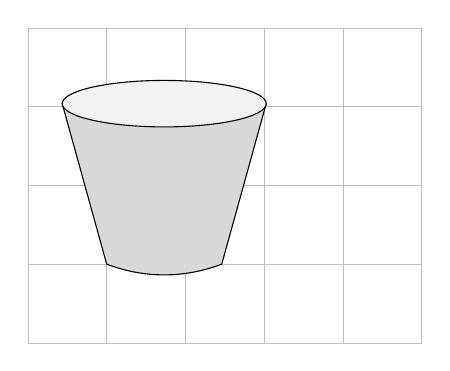
\begin{tikzpicture}

\pgfmathsetmacro{\acoor}{1.95 + random(1,3)*rnd}
\pgfmathsetmacro{\bcoor}{\acoor + rnd}
\pgfmathsetmacro{\ccoor}{.5 + .5*\acoor}
\pgfmathsetmacro{\first}{1 + (.4*\acoor - .5)}
\pgfmathsetmacro{\second}{1 + (.6*\acoor - .5)}
\pgfmathsetmacro{\split}{(2*\bcoor - 1 - \acoor)/2}
\pgfmathsetmacro{\ycoor}{1.5 + 2*rnd}
\pgfmathsetmacro{\corr}{.075 * \ycoor}
\pgfmathsetmacro{\abcorr}{(.08*(\bcoor - 1)) + .0065* \ycoor}


\draw [help lines,lightgray] (0,0) grid (5,4) ;
\draw[fill=gray!30] (1,1) .. controls (\first,1 - \abcorr) and (\second,1 - \abcorr) .. (\acoor,1) -- (\bcoor,\ycoor) --  (1 + \acoor - \bcoor,\ycoor) -- (1,1) ;
\draw[fill=gray!10] (\ccoor,\ycoor) ellipse (\split cm and \split*\corr cm) ;

\end{tikzpicture}
}

}


\newsavebox{\fifty}
\savebox{\fifty}{

\scalebox{4}{

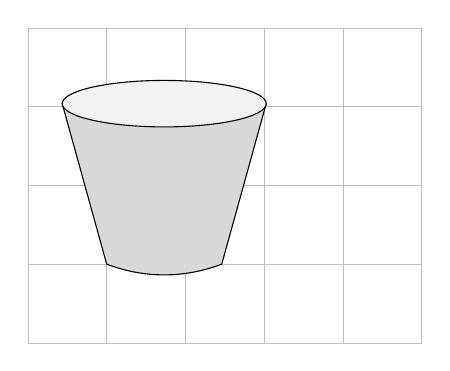
\begin{tikzpicture}

\pgfmathsetmacro{\acoor}{1.95 + random(1,3)*rnd}
\pgfmathsetmacro{\bcoor}{\acoor + rnd}
\pgfmathsetmacro{\ccoor}{.5 + .5*\acoor}
\pgfmathsetmacro{\first}{1 + (.4*\acoor - .5)}
\pgfmathsetmacro{\second}{1 + (.6*\acoor - .5)}
\pgfmathsetmacro{\split}{(2*\bcoor - 1 - \acoor)/2}
\pgfmathsetmacro{\ycoor}{1.5 + 2*rnd}
\pgfmathsetmacro{\corr}{.075 * \ycoor}
\pgfmathsetmacro{\abcorr}{(.08*(\bcoor - 1)) + .0065* \ycoor}


\draw [help lines,lightgray] (0,0) grid (5,4) ;
\draw[fill=gray!30] (1,1) .. controls (\first,1 - \abcorr) and (\second,1 - \abcorr) .. (\acoor,1) -- (\bcoor,\ycoor) --  (1 + \acoor - \bcoor,\ycoor) -- (1,1) ;
\draw[fill=gray!10] (\ccoor,\ycoor) ellipse (\split cm and \split*\corr cm) ;

\end{tikzpicture}
}

}

\newsavebox{\fiftyone}
\savebox{\fiftyone}{

\scalebox{4}{

\begin{tikzpicture}

\pgfmathsetmacro{\acoor}{1.95 + random(1,3)*rnd}
\pgfmathsetmacro{\bcoor}{\acoor + rnd}
\pgfmathsetmacro{\ccoor}{.5 + .5*\acoor}
\pgfmathsetmacro{\first}{1 + (.4*\acoor - .5)}
\pgfmathsetmacro{\second}{1 + (.6*\acoor - .5)}
\pgfmathsetmacro{\split}{(2*\bcoor - 1 - \acoor)/2}
\pgfmathsetmacro{\ycoor}{1.5 + 2*rnd}
\pgfmathsetmacro{\corr}{.075 * \ycoor}
\pgfmathsetmacro{\abcorr}{(.08*(\bcoor - 1)) + .0065* \ycoor}


\draw [help lines,lightgray] (0,0) grid (5,4) ;
\draw[fill=gray!30] (1,1) .. controls (\first,1 - \abcorr) and (\second,1 - \abcorr) .. (\acoor,1) -- (\bcoor,\ycoor) --  (1 + \acoor - \bcoor,\ycoor) -- (1,1) ;
\draw[fill=gray!10] (\ccoor,\ycoor) ellipse (\split cm and \split*\corr cm) ;

\end{tikzpicture}
}

}

\newsavebox{\fiftytwo}
\savebox{\fiftytwo}{

\scalebox{4}{

\begin{tikzpicture}

\pgfmathsetmacro{\acoor}{1.95 + random(1,3)*rnd}
\pgfmathsetmacro{\bcoor}{\acoor + rnd}
\pgfmathsetmacro{\ccoor}{.5 + .5*\acoor}
\pgfmathsetmacro{\first}{1 + (.4*\acoor - .5)}
\pgfmathsetmacro{\second}{1 + (.6*\acoor - .5)}
\pgfmathsetmacro{\split}{(2*\bcoor - 1 - \acoor)/2}
\pgfmathsetmacro{\ycoor}{1.5 + 2*rnd}
\pgfmathsetmacro{\corr}{.075 * \ycoor}
\pgfmathsetmacro{\abcorr}{(.08*(\bcoor - 1)) + .0065* \ycoor}


\draw [help lines,lightgray] (0,0) grid (5,4) ;
\draw[fill=gray!30] (1,1) .. controls (\first,1 - \abcorr) and (\second,1 - \abcorr) .. (\acoor,1) -- (\bcoor,\ycoor) --  (1 + \acoor - \bcoor,\ycoor) -- (1,1) ;
\draw[fill=gray!10] (\ccoor,\ycoor) ellipse (\split cm and \split*\corr cm) ;

\end{tikzpicture}
}

}

\newsavebox{\fiftythree}
\savebox{\fiftythree}{

\scalebox{4}{

\begin{tikzpicture}

\pgfmathsetmacro{\acoor}{1.95 + random(1,3)*rnd}
\pgfmathsetmacro{\bcoor}{\acoor + rnd}
\pgfmathsetmacro{\ccoor}{.5 + .5*\acoor}
\pgfmathsetmacro{\first}{1 + (.4*\acoor - .5)}
\pgfmathsetmacro{\second}{1 + (.6*\acoor - .5)}
\pgfmathsetmacro{\split}{(2*\bcoor - 1 - \acoor)/2}
\pgfmathsetmacro{\ycoor}{1.5 + 2*rnd}
\pgfmathsetmacro{\corr}{.075 * \ycoor}
\pgfmathsetmacro{\abcorr}{(.08*(\bcoor - 1)) + .0065* \ycoor}


\draw [help lines,lightgray] (0,0) grid (5,4) ;
\draw[fill=gray!30] (1,1) .. controls (\first,1 - \abcorr) and (\second,1 - \abcorr) .. (\acoor,1) -- (\bcoor,\ycoor) --  (1 + \acoor - \bcoor,\ycoor) -- (1,1) ;
\draw[fill=gray!10] (\ccoor,\ycoor) ellipse (\split cm and \split*\corr cm) ;

\end{tikzpicture}
}

}

\newsavebox{\fiftyfour}
\savebox{\fiftyfour}{

\scalebox{4}{

\begin{tikzpicture}

\pgfmathsetmacro{\acoor}{1.95 + random(1,3)*rnd}
\pgfmathsetmacro{\bcoor}{\acoor + rnd}
\pgfmathsetmacro{\ccoor}{.5 + .5*\acoor}
\pgfmathsetmacro{\first}{1 + (.4*\acoor - .5)}
\pgfmathsetmacro{\second}{1 + (.6*\acoor - .5)}
\pgfmathsetmacro{\split}{(2*\bcoor - 1 - \acoor)/2}
\pgfmathsetmacro{\ycoor}{1.5 + 2*rnd}
\pgfmathsetmacro{\corr}{.075 * \ycoor}
\pgfmathsetmacro{\abcorr}{(.08*(\bcoor - 1)) + .0065* \ycoor}


\draw [help lines,lightgray] (0,0) grid (5,4) ;
\draw[fill=gray!30] (1,1) .. controls (\first,1 - \abcorr) and (\second,1 - \abcorr) .. (\acoor,1) -- (\bcoor,\ycoor) --  (1 + \acoor - \bcoor,\ycoor) -- (1,1) ;
\draw[fill=gray!10] (\ccoor,\ycoor) ellipse (\split cm and \split*\corr cm) ;

\end{tikzpicture}
}

}

\newsavebox{\fiftyfive}
\savebox{\fiftyfive}{

\scalebox{4}{

\begin{tikzpicture}

\pgfmathsetmacro{\acoor}{1.95 + random(1,3)*rnd}
\pgfmathsetmacro{\bcoor}{\acoor + rnd}
\pgfmathsetmacro{\ccoor}{.5 + .5*\acoor}
\pgfmathsetmacro{\first}{1 + (.4*\acoor - .5)}
\pgfmathsetmacro{\second}{1 + (.6*\acoor - .5)}
\pgfmathsetmacro{\split}{(2*\bcoor - 1 - \acoor)/2}
\pgfmathsetmacro{\ycoor}{1.5 + 2*rnd}
\pgfmathsetmacro{\corr}{.075 * \ycoor}
\pgfmathsetmacro{\abcorr}{(.08*(\bcoor - 1)) + .0065* \ycoor}


\draw [help lines,lightgray] (0,0) grid (5,4) ;
\draw[fill=gray!30] (1,1) .. controls (\first,1 - \abcorr) and (\second,1 - \abcorr) .. (\acoor,1) -- (\bcoor,\ycoor) --  (1 + \acoor - \bcoor,\ycoor) -- (1,1) ;
\draw[fill=gray!10] (\ccoor,\ycoor) ellipse (\split cm and \split*\corr cm) ;

\end{tikzpicture}
}

}

\newsavebox{\fiftysix}
\savebox{\fiftysix}{

\scalebox{4}{

\begin{tikzpicture}

\pgfmathsetmacro{\acoor}{1.95 + random(1,3)*rnd}
\pgfmathsetmacro{\bcoor}{\acoor + rnd}
\pgfmathsetmacro{\ccoor}{.5 + .5*\acoor}
\pgfmathsetmacro{\first}{1 + (.4*\acoor - .5)}
\pgfmathsetmacro{\second}{1 + (.6*\acoor - .5)}
\pgfmathsetmacro{\split}{(2*\bcoor - 1 - \acoor)/2}
\pgfmathsetmacro{\ycoor}{1.5 + 2*rnd}
\pgfmathsetmacro{\corr}{.075 * \ycoor}
\pgfmathsetmacro{\abcorr}{(.08*(\bcoor - 1)) + .0065* \ycoor}


\draw [help lines,lightgray] (0,0) grid (5,4) ;
\draw[fill=gray!30] (1,1) .. controls (\first,1 - \abcorr) and (\second,1 - \abcorr) .. (\acoor,1) -- (\bcoor,\ycoor) --  (1 + \acoor - \bcoor,\ycoor) -- (1,1) ;
\draw[fill=gray!10] (\ccoor,\ycoor) ellipse (\split cm and \split*\corr cm) ;

\end{tikzpicture}
}

}

\newsavebox{\fiftyseven}
\savebox{\fiftyseven}{

\scalebox{4}{

\begin{tikzpicture}

\pgfmathsetmacro{\acoor}{1.95 + random(1,3)*rnd}
\pgfmathsetmacro{\bcoor}{\acoor + rnd}
\pgfmathsetmacro{\ccoor}{.5 + .5*\acoor}
\pgfmathsetmacro{\first}{1 + (.4*\acoor - .5)}
\pgfmathsetmacro{\second}{1 + (.6*\acoor - .5)}
\pgfmathsetmacro{\split}{(2*\bcoor - 1 - \acoor)/2}
\pgfmathsetmacro{\ycoor}{1.5 + 2*rnd}
\pgfmathsetmacro{\corr}{.075 * \ycoor}
\pgfmathsetmacro{\abcorr}{(.08*(\bcoor - 1)) + .0065* \ycoor}


\draw [help lines,lightgray] (0,0) grid (5,4) ;
\draw[fill=gray!30] (1,1) .. controls (\first,1 - \abcorr) and (\second,1 - \abcorr) .. (\acoor,1) -- (\bcoor,\ycoor) --  (1 + \acoor - \bcoor,\ycoor) -- (1,1) ;
\draw[fill=gray!10] (\ccoor,\ycoor) ellipse (\split cm and \split*\corr cm) ;

\end{tikzpicture}
}

}

\newsavebox{\fiftyeight}
\savebox{\fiftyeight}{

\scalebox{4}{

\begin{tikzpicture}

\pgfmathsetmacro{\acoor}{1.95 + random(1,3)*rnd}
\pgfmathsetmacro{\bcoor}{\acoor + rnd}
\pgfmathsetmacro{\ccoor}{.5 + .5*\acoor}
\pgfmathsetmacro{\first}{1 + (.4*\acoor - .5)}
\pgfmathsetmacro{\second}{1 + (.6*\acoor - .5)}
\pgfmathsetmacro{\split}{(2*\bcoor - 1 - \acoor)/2}
\pgfmathsetmacro{\ycoor}{1.5 + 2*rnd}
\pgfmathsetmacro{\corr}{.075 * \ycoor}
\pgfmathsetmacro{\abcorr}{(.08*(\bcoor - 1)) + .0065* \ycoor}


\draw [help lines,lightgray] (0,0) grid (5,4) ;
\draw[fill=gray!30] (1,1) .. controls (\first,1 - \abcorr) and (\second,1 - \abcorr) .. (\acoor,1) -- (\bcoor,\ycoor) --  (1 + \acoor - \bcoor,\ycoor) -- (1,1) ;
\draw[fill=gray!10] (\ccoor,\ycoor) ellipse (\split cm and \split*\corr cm) ;

\end{tikzpicture}
}

}

\newsavebox{\fiftynine}
\savebox{\fiftynine}{

\scalebox{4}{

\begin{tikzpicture}

\pgfmathsetmacro{\acoor}{1.95 + random(1,3)*rnd}
\pgfmathsetmacro{\bcoor}{\acoor + rnd}
\pgfmathsetmacro{\ccoor}{.5 + .5*\acoor}
\pgfmathsetmacro{\first}{1 + (.4*\acoor - .5)}
\pgfmathsetmacro{\second}{1 + (.6*\acoor - .5)}
\pgfmathsetmacro{\split}{(2*\bcoor - 1 - \acoor)/2}
\pgfmathsetmacro{\ycoor}{1.5 + 2*rnd}
\pgfmathsetmacro{\corr}{.075 * \ycoor}
\pgfmathsetmacro{\abcorr}{(.08*(\bcoor - 1)) + .0065* \ycoor}


\draw [help lines,lightgray] (0,0) grid (5,4) ;
\draw[fill=gray!30] (1,1) .. controls (\first,1 - \abcorr) and (\second,1 - \abcorr) .. (\acoor,1) -- (\bcoor,\ycoor) --  (1 + \acoor - \bcoor,\ycoor) -- (1,1) ;
\draw[fill=gray!10] (\ccoor,\ycoor) ellipse (\split cm and \split*\corr cm) ;

\end{tikzpicture}
}

}


\newsavebox{\sixty}
\savebox{\sixty}{

\scalebox{4}{

\begin{tikzpicture}

\pgfmathsetmacro{\acoor}{1.95 + random(1,3)*rnd}
\pgfmathsetmacro{\bcoor}{\acoor + rnd}
\pgfmathsetmacro{\ccoor}{.5 + .5*\acoor}
\pgfmathsetmacro{\first}{1 + (.4*\acoor - .5)}
\pgfmathsetmacro{\second}{1 + (.6*\acoor - .5)}
\pgfmathsetmacro{\split}{(2*\bcoor - 1 - \acoor)/2}
\pgfmathsetmacro{\ycoor}{1.5 + 2*rnd}
\pgfmathsetmacro{\corr}{.075 * \ycoor}
\pgfmathsetmacro{\abcorr}{(.08*(\bcoor - 1)) + .0065* \ycoor}


\draw [help lines,lightgray] (0,0) grid (5,4) ;
\draw[fill=gray!30] (1,1) .. controls (\first,1 - \abcorr) and (\second,1 - \abcorr) .. (\acoor,1) -- (\bcoor,\ycoor) --  (1 + \acoor - \bcoor,\ycoor) -- (1,1) ;
\draw[fill=gray!10] (\ccoor,\ycoor) ellipse (\split cm and \split*\corr cm) ;

\end{tikzpicture}
}

}

\newsavebox{\sixtyone}
\savebox{\sixtyone}{

\scalebox{4}{

\begin{tikzpicture}

\pgfmathsetmacro{\acoor}{1.95 + random(1,3)*rnd}
\pgfmathsetmacro{\bcoor}{\acoor + rnd}
\pgfmathsetmacro{\ccoor}{.5 + .5*\acoor}
\pgfmathsetmacro{\first}{1 + (.4*\acoor - .5)}
\pgfmathsetmacro{\second}{1 + (.6*\acoor - .5)}
\pgfmathsetmacro{\split}{(2*\bcoor - 1 - \acoor)/2}
\pgfmathsetmacro{\ycoor}{1.5 + 2*rnd}
\pgfmathsetmacro{\corr}{.075 * \ycoor}
\pgfmathsetmacro{\abcorr}{(.08*(\bcoor - 1)) + .0065* \ycoor}


\draw [help lines,lightgray] (0,0) grid (5,4) ;
\draw[fill=gray!30] (1,1) .. controls (\first,1 - \abcorr) and (\second,1 - \abcorr) .. (\acoor,1) -- (\bcoor,\ycoor) --  (1 + \acoor - \bcoor,\ycoor) -- (1,1) ;
\draw[fill=gray!10] (\ccoor,\ycoor) ellipse (\split cm and \split*\corr cm) ;

\end{tikzpicture}
}

}

\newsavebox{\sixtytwo}
\savebox{\sixtytwo}{

\scalebox{4}{

\begin{tikzpicture}

\pgfmathsetmacro{\acoor}{1.95 + random(1,3)*rnd}
\pgfmathsetmacro{\bcoor}{\acoor + rnd}
\pgfmathsetmacro{\ccoor}{.5 + .5*\acoor}
\pgfmathsetmacro{\first}{1 + (.4*\acoor - .5)}
\pgfmathsetmacro{\second}{1 + (.6*\acoor - .5)}
\pgfmathsetmacro{\split}{(2*\bcoor - 1 - \acoor)/2}
\pgfmathsetmacro{\ycoor}{1.5 + 2*rnd}
\pgfmathsetmacro{\corr}{.075 * \ycoor}
\pgfmathsetmacro{\abcorr}{(.08*(\bcoor - 1)) + .0065* \ycoor}


\draw [help lines,lightgray] (0,0) grid (5,4) ;
\draw[fill=gray!30] (1,1) .. controls (\first,1 - \abcorr) and (\second,1 - \abcorr) .. (\acoor,1) -- (\bcoor,\ycoor) --  (1 + \acoor - \bcoor,\ycoor) -- (1,1) ;
\draw[fill=gray!10] (\ccoor,\ycoor) ellipse (\split cm and \split*\corr cm) ;

\end{tikzpicture}
}

}

\newsavebox{\sixtythree}
\savebox{\sixtythree}{

\scalebox{4}{

\begin{tikzpicture}

\pgfmathsetmacro{\acoor}{1.95 + random(1,3)*rnd}
\pgfmathsetmacro{\bcoor}{\acoor + rnd}
\pgfmathsetmacro{\ccoor}{.5 + .5*\acoor}
\pgfmathsetmacro{\first}{1 + (.4*\acoor - .5)}
\pgfmathsetmacro{\second}{1 + (.6*\acoor - .5)}
\pgfmathsetmacro{\split}{(2*\bcoor - 1 - \acoor)/2}
\pgfmathsetmacro{\ycoor}{1.5 + 2*rnd}
\pgfmathsetmacro{\corr}{.075 * \ycoor}
\pgfmathsetmacro{\abcorr}{(.08*(\bcoor - 1)) + .0065* \ycoor}


\draw [help lines,lightgray] (0,0) grid (5,4) ;
\draw[fill=gray!30] (1,1) .. controls (\first,1 - \abcorr) and (\second,1 - \abcorr) .. (\acoor,1) -- (\bcoor,\ycoor) --  (1 + \acoor - \bcoor,\ycoor) -- (1,1) ;
\draw[fill=gray!10] (\ccoor,\ycoor) ellipse (\split cm and \split*\corr cm) ;

\end{tikzpicture}
}

}

\newsavebox{\sixtyfour}
\savebox{\sixtyfour}{

\scalebox{4}{

\begin{tikzpicture}

\pgfmathsetmacro{\acoor}{1.95 + random(1,3)*rnd}
\pgfmathsetmacro{\bcoor}{\acoor + rnd}
\pgfmathsetmacro{\ccoor}{.5 + .5*\acoor}
\pgfmathsetmacro{\first}{1 + (.4*\acoor - .5)}
\pgfmathsetmacro{\second}{1 + (.6*\acoor - .5)}
\pgfmathsetmacro{\split}{(2*\bcoor - 1 - \acoor)/2}
\pgfmathsetmacro{\ycoor}{1.5 + 2*rnd}
\pgfmathsetmacro{\corr}{.075 * \ycoor}
\pgfmathsetmacro{\abcorr}{(.08*(\bcoor - 1)) + .0065* \ycoor}


\draw [help lines,lightgray] (0,0) grid (5,4) ;
\draw[fill=gray!30] (1,1) .. controls (\first,1 - \abcorr) and (\second,1 - \abcorr) .. (\acoor,1) -- (\bcoor,\ycoor) --  (1 + \acoor - \bcoor,\ycoor) -- (1,1) ;
\draw[fill=gray!10] (\ccoor,\ycoor) ellipse (\split cm and \split*\corr cm) ;

\end{tikzpicture}
}

}

\newsavebox{\sixtyfive}
\savebox{\sixtyfive}{

\scalebox{4}{

\begin{tikzpicture}

\pgfmathsetmacro{\acoor}{1.95 + random(1,3)*rnd}
\pgfmathsetmacro{\bcoor}{\acoor + rnd}
\pgfmathsetmacro{\ccoor}{.5 + .5*\acoor}
\pgfmathsetmacro{\first}{1 + (.4*\acoor - .5)}
\pgfmathsetmacro{\second}{1 + (.6*\acoor - .5)}
\pgfmathsetmacro{\split}{(2*\bcoor - 1 - \acoor)/2}
\pgfmathsetmacro{\ycoor}{1.5 + 2*rnd}
\pgfmathsetmacro{\corr}{.075 * \ycoor}
\pgfmathsetmacro{\abcorr}{(.08*(\bcoor - 1)) + .0065* \ycoor}


\draw [help lines,lightgray] (0,0) grid (5,4) ;
\draw[fill=gray!30] (1,1) .. controls (\first,1 - \abcorr) and (\second,1 - \abcorr) .. (\acoor,1) -- (\bcoor,\ycoor) --  (1 + \acoor - \bcoor,\ycoor) -- (1,1) ;
\draw[fill=gray!10] (\ccoor,\ycoor) ellipse (\split cm and \split*\corr cm) ;

\end{tikzpicture}
}

}

\newsavebox{\sixtysix}
\savebox{\sixtysix}{

\scalebox{4}{

\begin{tikzpicture}

\pgfmathsetmacro{\acoor}{1.95 + random(1,3)*rnd}
\pgfmathsetmacro{\bcoor}{\acoor + rnd}
\pgfmathsetmacro{\ccoor}{.5 + .5*\acoor}
\pgfmathsetmacro{\first}{1 + (.4*\acoor - .5)}
\pgfmathsetmacro{\second}{1 + (.6*\acoor - .5)}
\pgfmathsetmacro{\split}{(2*\bcoor - 1 - \acoor)/2}
\pgfmathsetmacro{\ycoor}{1.5 + 2*rnd}
\pgfmathsetmacro{\corr}{.075 * \ycoor}
\pgfmathsetmacro{\abcorr}{(.08*(\bcoor - 1)) + .0065* \ycoor}


\draw [help lines,lightgray] (0,0) grid (5,4) ;
\draw[fill=gray!30] (1,1) .. controls (\first,1 - \abcorr) and (\second,1 - \abcorr) .. (\acoor,1) -- (\bcoor,\ycoor) --  (1 + \acoor - \bcoor,\ycoor) -- (1,1) ;
\draw[fill=gray!10] (\ccoor,\ycoor) ellipse (\split cm and \split*\corr cm) ;

\end{tikzpicture}
}

}

\newsavebox{\sixtyseven}
\savebox{\sixtyseven}{

\scalebox{4}{

\begin{tikzpicture}

\pgfmathsetmacro{\acoor}{1.95 + random(1,3)*rnd}
\pgfmathsetmacro{\bcoor}{\acoor + rnd}
\pgfmathsetmacro{\ccoor}{.5 + .5*\acoor}
\pgfmathsetmacro{\first}{1 + (.4*\acoor - .5)}
\pgfmathsetmacro{\second}{1 + (.6*\acoor - .5)}
\pgfmathsetmacro{\split}{(2*\bcoor - 1 - \acoor)/2}
\pgfmathsetmacro{\ycoor}{1.5 + 2*rnd}
\pgfmathsetmacro{\corr}{.075 * \ycoor}
\pgfmathsetmacro{\abcorr}{(.08*(\bcoor - 1)) + .0065* \ycoor}


\draw [help lines,lightgray] (0,0) grid (5,4) ;
\draw[fill=gray!30] (1,1) .. controls (\first,1 - \abcorr) and (\second,1 - \abcorr) .. (\acoor,1) -- (\bcoor,\ycoor) --  (1 + \acoor - \bcoor,\ycoor) -- (1,1) ;
\draw[fill=gray!10] (\ccoor,\ycoor) ellipse (\split cm and \split*\corr cm) ;

\end{tikzpicture}
}

}

\newsavebox{\sixtyeight}
\savebox{\sixtyeight}{

\scalebox{4}{

\begin{tikzpicture}

\pgfmathsetmacro{\acoor}{1.95 + random(1,3)*rnd}
\pgfmathsetmacro{\bcoor}{\acoor + rnd}
\pgfmathsetmacro{\ccoor}{.5 + .5*\acoor}
\pgfmathsetmacro{\first}{1 + (.4*\acoor - .5)}
\pgfmathsetmacro{\second}{1 + (.6*\acoor - .5)}
\pgfmathsetmacro{\split}{(2*\bcoor - 1 - \acoor)/2}
\pgfmathsetmacro{\ycoor}{1.5 + 2*rnd}
\pgfmathsetmacro{\corr}{.075 * \ycoor}
\pgfmathsetmacro{\abcorr}{(.08*(\bcoor - 1)) + .0065* \ycoor}


\draw [help lines,lightgray] (0,0) grid (5,4) ;
\draw[fill=gray!30] (1,1) .. controls (\first,1 - \abcorr) and (\second,1 - \abcorr) .. (\acoor,1) -- (\bcoor,\ycoor) --  (1 + \acoor - \bcoor,\ycoor) -- (1,1) ;
\draw[fill=gray!10] (\ccoor,\ycoor) ellipse (\split cm and \split*\corr cm) ;

\end{tikzpicture}
}

}

\newsavebox{\sixtynine}
\savebox{\sixtynine}{

\scalebox{4}{

\begin{tikzpicture}

\pgfmathsetmacro{\acoor}{1.95 + random(1,3)*rnd}
\pgfmathsetmacro{\bcoor}{\acoor + rnd}
\pgfmathsetmacro{\ccoor}{.5 + .5*\acoor}
\pgfmathsetmacro{\first}{1 + (.4*\acoor - .5)}
\pgfmathsetmacro{\second}{1 + (.6*\acoor - .5)}
\pgfmathsetmacro{\split}{(2*\bcoor - 1 - \acoor)/2}
\pgfmathsetmacro{\ycoor}{1.5 + 2*rnd}
\pgfmathsetmacro{\corr}{.075 * \ycoor}
\pgfmathsetmacro{\abcorr}{(.08*(\bcoor - 1)) + .0065* \ycoor}


\draw [help lines,lightgray] (0,0) grid (5,4) ;
\draw[fill=gray!30] (1,1) .. controls (\first,1 - \abcorr) and (\second,1 - \abcorr) .. (\acoor,1) -- (\bcoor,\ycoor) --  (1 + \acoor - \bcoor,\ycoor) -- (1,1) ;
\draw[fill=gray!10] (\ccoor,\ycoor) ellipse (\split cm and \split*\corr cm) ;

\end{tikzpicture}
}

}


\newsavebox{\seventy}
\savebox{\seventy}{

\scalebox{4}{

\begin{tikzpicture}

\pgfmathsetmacro{\acoor}{1.95 + random(1,3)*rnd}
\pgfmathsetmacro{\bcoor}{\acoor + rnd}
\pgfmathsetmacro{\ccoor}{.5 + .5*\acoor}
\pgfmathsetmacro{\first}{1 + (.4*\acoor - .5)}
\pgfmathsetmacro{\second}{1 + (.6*\acoor - .5)}
\pgfmathsetmacro{\split}{(2*\bcoor - 1 - \acoor)/2}
\pgfmathsetmacro{\ycoor}{1.5 + 2*rnd}
\pgfmathsetmacro{\corr}{.075 * \ycoor}
\pgfmathsetmacro{\abcorr}{(.08*(\bcoor - 1)) + .0065* \ycoor}


\draw [help lines,lightgray] (0,0) grid (5,4) ;
\draw[fill=gray!30] (1,1) .. controls (\first,1 - \abcorr) and (\second,1 - \abcorr) .. (\acoor,1) -- (\bcoor,\ycoor) --  (1 + \acoor - \bcoor,\ycoor) -- (1,1) ;
\draw[fill=gray!10] (\ccoor,\ycoor) ellipse (\split cm and \split*\corr cm) ;

\end{tikzpicture}
}

}

\newsavebox{\seventyone}
\savebox{\seventyone}{

\scalebox{4}{

\begin{tikzpicture}

\pgfmathsetmacro{\acoor}{1.95 + random(1,3)*rnd}
\pgfmathsetmacro{\bcoor}{\acoor + rnd}
\pgfmathsetmacro{\ccoor}{.5 + .5*\acoor}
\pgfmathsetmacro{\first}{1 + (.4*\acoor - .5)}
\pgfmathsetmacro{\second}{1 + (.6*\acoor - .5)}
\pgfmathsetmacro{\split}{(2*\bcoor - 1 - \acoor)/2}
\pgfmathsetmacro{\ycoor}{1.5 + 2*rnd}
\pgfmathsetmacro{\corr}{.075 * \ycoor}
\pgfmathsetmacro{\abcorr}{(.08*(\bcoor - 1)) + .0065* \ycoor}


\draw [help lines,lightgray] (0,0) grid (5,4) ;
\draw[fill=gray!30] (1,1) .. controls (\first,1 - \abcorr) and (\second,1 - \abcorr) .. (\acoor,1) -- (\bcoor,\ycoor) --  (1 + \acoor - \bcoor,\ycoor) -- (1,1) ;
\draw[fill=gray!10] (\ccoor,\ycoor) ellipse (\split cm and \split*\corr cm) ;

\end{tikzpicture}
}

}

\newsavebox{\seventytwo}
\savebox{\seventytwo}{

\scalebox{4}{

\begin{tikzpicture}

\pgfmathsetmacro{\acoor}{1.95 + random(1,3)*rnd}
\pgfmathsetmacro{\bcoor}{\acoor + rnd}
\pgfmathsetmacro{\ccoor}{.5 + .5*\acoor}
\pgfmathsetmacro{\first}{1 + (.4*\acoor - .5)}
\pgfmathsetmacro{\second}{1 + (.6*\acoor - .5)}
\pgfmathsetmacro{\split}{(2*\bcoor - 1 - \acoor)/2}
\pgfmathsetmacro{\ycoor}{1.5 + 2*rnd}
\pgfmathsetmacro{\corr}{.075 * \ycoor}
\pgfmathsetmacro{\abcorr}{(.08*(\bcoor - 1)) + .0065* \ycoor}


\draw [help lines,lightgray] (0,0) grid (5,4) ;
\draw[fill=gray!30] (1,1) .. controls (\first,1 - \abcorr) and (\second,1 - \abcorr) .. (\acoor,1) -- (\bcoor,\ycoor) --  (1 + \acoor - \bcoor,\ycoor) -- (1,1) ;
\draw[fill=gray!10] (\ccoor,\ycoor) ellipse (\split cm and \split*\corr cm) ;

\end{tikzpicture}
}

}

\newsavebox{\seventythree}
\savebox{\seventythree}{

\scalebox{4}{

\begin{tikzpicture}

\pgfmathsetmacro{\acoor}{1.95 + random(1,3)*rnd}
\pgfmathsetmacro{\bcoor}{\acoor + rnd}
\pgfmathsetmacro{\ccoor}{.5 + .5*\acoor}
\pgfmathsetmacro{\first}{1 + (.4*\acoor - .5)}
\pgfmathsetmacro{\second}{1 + (.6*\acoor - .5)}
\pgfmathsetmacro{\split}{(2*\bcoor - 1 - \acoor)/2}
\pgfmathsetmacro{\ycoor}{1.5 + 2*rnd}
\pgfmathsetmacro{\corr}{.075 * \ycoor}
\pgfmathsetmacro{\abcorr}{(.08*(\bcoor - 1)) + .0065* \ycoor}


\draw [help lines,lightgray] (0,0) grid (5,4) ;
\draw[fill=gray!30] (1,1) .. controls (\first,1 - \abcorr) and (\second,1 - \abcorr) .. (\acoor,1) -- (\bcoor,\ycoor) --  (1 + \acoor - \bcoor,\ycoor) -- (1,1) ;
\draw[fill=gray!10] (\ccoor,\ycoor) ellipse (\split cm and \split*\corr cm) ;

\end{tikzpicture}
}

}

\newsavebox{\seventyfour}
\savebox{\seventyfour}{

\scalebox{4}{

\begin{tikzpicture}

\pgfmathsetmacro{\acoor}{1.95 + random(1,3)*rnd}
\pgfmathsetmacro{\bcoor}{\acoor + rnd}
\pgfmathsetmacro{\ccoor}{.5 + .5*\acoor}
\pgfmathsetmacro{\first}{1 + (.4*\acoor - .5)}
\pgfmathsetmacro{\second}{1 + (.6*\acoor - .5)}
\pgfmathsetmacro{\split}{(2*\bcoor - 1 - \acoor)/2}
\pgfmathsetmacro{\ycoor}{1.5 + 2*rnd}
\pgfmathsetmacro{\corr}{.075 * \ycoor}
\pgfmathsetmacro{\abcorr}{(.08*(\bcoor - 1)) + .0065* \ycoor}


\draw [help lines,lightgray] (0,0) grid (5,4) ;
\draw[fill=gray!30] (1,1) .. controls (\first,1 - \abcorr) and (\second,1 - \abcorr) .. (\acoor,1) -- (\bcoor,\ycoor) --  (1 + \acoor - \bcoor,\ycoor) -- (1,1) ;
\draw[fill=gray!10] (\ccoor,\ycoor) ellipse (\split cm and \split*\corr cm) ;

\end{tikzpicture}
}

}

\newsavebox{\seventyfive}
\savebox{\seventyfive}{

\scalebox{4}{

\begin{tikzpicture}

\pgfmathsetmacro{\acoor}{1.95 + random(1,3)*rnd}
\pgfmathsetmacro{\bcoor}{\acoor + rnd}
\pgfmathsetmacro{\ccoor}{.5 + .5*\acoor}
\pgfmathsetmacro{\first}{1 + (.4*\acoor - .5)}
\pgfmathsetmacro{\second}{1 + (.6*\acoor - .5)}
\pgfmathsetmacro{\split}{(2*\bcoor - 1 - \acoor)/2}
\pgfmathsetmacro{\ycoor}{1.5 + 2*rnd}
\pgfmathsetmacro{\corr}{.075 * \ycoor}
\pgfmathsetmacro{\abcorr}{(.08*(\bcoor - 1)) + .0065* \ycoor}


\draw [help lines,lightgray] (0,0) grid (5,4) ;
\draw[fill=gray!30] (1,1) .. controls (\first,1 - \abcorr) and (\second,1 - \abcorr) .. (\acoor,1) -- (\bcoor,\ycoor) --  (1 + \acoor - \bcoor,\ycoor) -- (1,1) ;
\draw[fill=gray!10] (\ccoor,\ycoor) ellipse (\split cm and \split*\corr cm) ;

\end{tikzpicture}
}

}

\newsavebox{\seventysix}
\savebox{\seventysix}{

\scalebox{4}{

\begin{tikzpicture}

\pgfmathsetmacro{\acoor}{1.95 + random(1,3)*rnd}
\pgfmathsetmacro{\bcoor}{\acoor + rnd}
\pgfmathsetmacro{\ccoor}{.5 + .5*\acoor}
\pgfmathsetmacro{\first}{1 + (.4*\acoor - .5)}
\pgfmathsetmacro{\second}{1 + (.6*\acoor - .5)}
\pgfmathsetmacro{\split}{(2*\bcoor - 1 - \acoor)/2}
\pgfmathsetmacro{\ycoor}{1.5 + 2*rnd}
\pgfmathsetmacro{\corr}{.075 * \ycoor}
\pgfmathsetmacro{\abcorr}{(.08*(\bcoor - 1)) + .0065* \ycoor}


\draw [help lines,lightgray] (0,0) grid (5,4) ;
\draw[fill=gray!30] (1,1) .. controls (\first,1 - \abcorr) and (\second,1 - \abcorr) .. (\acoor,1) -- (\bcoor,\ycoor) --  (1 + \acoor - \bcoor,\ycoor) -- (1,1) ;
\draw[fill=gray!10] (\ccoor,\ycoor) ellipse (\split cm and \split*\corr cm) ;

\end{tikzpicture}
}

}

\newsavebox{\seventyseven}
\savebox{\seventyseven}{

\scalebox{4}{

\begin{tikzpicture}

\pgfmathsetmacro{\acoor}{1.95 + random(1,3)*rnd}
\pgfmathsetmacro{\bcoor}{\acoor + rnd}
\pgfmathsetmacro{\ccoor}{.5 + .5*\acoor}
\pgfmathsetmacro{\first}{1 + (.4*\acoor - .5)}
\pgfmathsetmacro{\second}{1 + (.6*\acoor - .5)}
\pgfmathsetmacro{\split}{(2*\bcoor - 1 - \acoor)/2}
\pgfmathsetmacro{\ycoor}{1.5 + 2*rnd}
\pgfmathsetmacro{\corr}{.075 * \ycoor}
\pgfmathsetmacro{\abcorr}{(.08*(\bcoor - 1)) + .0065* \ycoor}


\draw [help lines,lightgray] (0,0) grid (5,4) ;
\draw[fill=gray!30] (1,1) .. controls (\first,1 - \abcorr) and (\second,1 - \abcorr) .. (\acoor,1) -- (\bcoor,\ycoor) --  (1 + \acoor - \bcoor,\ycoor) -- (1,1) ;
\draw[fill=gray!10] (\ccoor,\ycoor) ellipse (\split cm and \split*\corr cm) ;

\end{tikzpicture}
}

}

\newsavebox{\seventyeight}
\savebox{\seventyeight}{

\scalebox{4}{

\begin{tikzpicture}

\pgfmathsetmacro{\acoor}{1.95 + random(1,3)*rnd}
\pgfmathsetmacro{\bcoor}{\acoor + rnd}
\pgfmathsetmacro{\ccoor}{.5 + .5*\acoor}
\pgfmathsetmacro{\first}{1 + (.4*\acoor - .5)}
\pgfmathsetmacro{\second}{1 + (.6*\acoor - .5)}
\pgfmathsetmacro{\split}{(2*\bcoor - 1 - \acoor)/2}
\pgfmathsetmacro{\ycoor}{1.5 + 2*rnd}
\pgfmathsetmacro{\corr}{.075 * \ycoor}
\pgfmathsetmacro{\abcorr}{(.08*(\bcoor - 1)) + .0065* \ycoor}


\draw [help lines,lightgray] (0,0) grid (5,4) ;
\draw[fill=gray!30] (1,1) .. controls (\first,1 - \abcorr) and (\second,1 - \abcorr) .. (\acoor,1) -- (\bcoor,\ycoor) --  (1 + \acoor - \bcoor,\ycoor) -- (1,1) ;
\draw[fill=gray!10] (\ccoor,\ycoor) ellipse (\split cm and \split*\corr cm) ;

\end{tikzpicture}
}

}

\newsavebox{\seventynine}
\savebox{\seventynine}{

\scalebox{4}{

\begin{tikzpicture}

\pgfmathsetmacro{\acoor}{1.95 + random(1,3)*rnd}
\pgfmathsetmacro{\bcoor}{\acoor + rnd}
\pgfmathsetmacro{\ccoor}{.5 + .5*\acoor}
\pgfmathsetmacro{\first}{1 + (.4*\acoor - .5)}
\pgfmathsetmacro{\second}{1 + (.6*\acoor - .5)}
\pgfmathsetmacro{\split}{(2*\bcoor - 1 - \acoor)/2}
\pgfmathsetmacro{\ycoor}{1.5 + 2*rnd}
\pgfmathsetmacro{\corr}{.075 * \ycoor}
\pgfmathsetmacro{\abcorr}{(.08*(\bcoor - 1)) + .0065* \ycoor}


\draw [help lines,lightgray] (0,0) grid (5,4) ;
\draw[fill=gray!30] (1,1) .. controls (\first,1 - \abcorr) and (\second,1 - \abcorr) .. (\acoor,1) -- (\bcoor,\ycoor) --  (1 + \acoor - \bcoor,\ycoor) -- (1,1) ;
\draw[fill=gray!10] (\ccoor,\ycoor) ellipse (\split cm and \split*\corr cm) ;

\end{tikzpicture}
}

}


\newsavebox{\eighty}
\savebox{\eighty}{

\scalebox{4}{

\begin{tikzpicture}

\pgfmathsetmacro{\acoor}{1.95 + random(1,3)*rnd}
\pgfmathsetmacro{\bcoor}{\acoor + rnd}
\pgfmathsetmacro{\ccoor}{.5 + .5*\acoor}
\pgfmathsetmacro{\first}{1 + (.4*\acoor - .5)}
\pgfmathsetmacro{\second}{1 + (.6*\acoor - .5)}
\pgfmathsetmacro{\split}{(2*\bcoor - 1 - \acoor)/2}
\pgfmathsetmacro{\ycoor}{1.5 + 2*rnd}
\pgfmathsetmacro{\corr}{.075 * \ycoor}
\pgfmathsetmacro{\abcorr}{(.08*(\bcoor - 1)) + .0065* \ycoor}


\draw [help lines,lightgray] (0,0) grid (5,4) ;
\draw[fill=gray!30] (1,1) .. controls (\first,1 - \abcorr) and (\second,1 - \abcorr) .. (\acoor,1) -- (\bcoor,\ycoor) --  (1 + \acoor - \bcoor,\ycoor) -- (1,1) ;
\draw[fill=gray!10] (\ccoor,\ycoor) ellipse (\split cm and \split*\corr cm) ;

\end{tikzpicture}
}

}

\newsavebox{\eightyone}
\savebox{\eightyone}{

\scalebox{4}{

\begin{tikzpicture}

\pgfmathsetmacro{\acoor}{1.95 + random(1,3)*rnd}
\pgfmathsetmacro{\bcoor}{\acoor + rnd}
\pgfmathsetmacro{\ccoor}{.5 + .5*\acoor}
\pgfmathsetmacro{\first}{1 + (.4*\acoor - .5)}
\pgfmathsetmacro{\second}{1 + (.6*\acoor - .5)}
\pgfmathsetmacro{\split}{(2*\bcoor - 1 - \acoor)/2}
\pgfmathsetmacro{\ycoor}{1.5 + 2*rnd}
\pgfmathsetmacro{\corr}{.075 * \ycoor}
\pgfmathsetmacro{\abcorr}{(.08*(\bcoor - 1)) + .0065* \ycoor}


\draw [help lines,lightgray] (0,0) grid (5,4) ;
\draw[fill=gray!30] (1,1) .. controls (\first,1 - \abcorr) and (\second,1 - \abcorr) .. (\acoor,1) -- (\bcoor,\ycoor) --  (1 + \acoor - \bcoor,\ycoor) -- (1,1) ;
\draw[fill=gray!10] (\ccoor,\ycoor) ellipse (\split cm and \split*\corr cm) ;

\end{tikzpicture}
}

}

\newsavebox{\eightytwo}
\savebox{\eightytwo}{

\scalebox{4}{

\begin{tikzpicture}

\pgfmathsetmacro{\acoor}{1.95 + random(1,3)*rnd}
\pgfmathsetmacro{\bcoor}{\acoor + rnd}
\pgfmathsetmacro{\ccoor}{.5 + .5*\acoor}
\pgfmathsetmacro{\first}{1 + (.4*\acoor - .5)}
\pgfmathsetmacro{\second}{1 + (.6*\acoor - .5)}
\pgfmathsetmacro{\split}{(2*\bcoor - 1 - \acoor)/2}
\pgfmathsetmacro{\ycoor}{1.5 + 2*rnd}
\pgfmathsetmacro{\corr}{.075 * \ycoor}
\pgfmathsetmacro{\abcorr}{(.08*(\bcoor - 1)) + .0065* \ycoor}


\draw [help lines,lightgray] (0,0) grid (5,4) ;
\draw[fill=gray!30] (1,1) .. controls (\first,1 - \abcorr) and (\second,1 - \abcorr) .. (\acoor,1) -- (\bcoor,\ycoor) --  (1 + \acoor - \bcoor,\ycoor) -- (1,1) ;
\draw[fill=gray!10] (\ccoor,\ycoor) ellipse (\split cm and \split*\corr cm) ;

\end{tikzpicture}
}

}

\newsavebox{\eightythree}
\savebox{\eightythree}{

\scalebox{4}{

\begin{tikzpicture}

\pgfmathsetmacro{\acoor}{1.95 + random(1,3)*rnd}
\pgfmathsetmacro{\bcoor}{\acoor + rnd}
\pgfmathsetmacro{\ccoor}{.5 + .5*\acoor}
\pgfmathsetmacro{\first}{1 + (.4*\acoor - .5)}
\pgfmathsetmacro{\second}{1 + (.6*\acoor - .5)}
\pgfmathsetmacro{\split}{(2*\bcoor - 1 - \acoor)/2}
\pgfmathsetmacro{\ycoor}{1.5 + 2*rnd}
\pgfmathsetmacro{\corr}{.075 * \ycoor}
\pgfmathsetmacro{\abcorr}{(.08*(\bcoor - 1)) + .0065* \ycoor}


\draw [help lines,lightgray] (0,0) grid (5,4) ;
\draw[fill=gray!30] (1,1) .. controls (\first,1 - \abcorr) and (\second,1 - \abcorr) .. (\acoor,1) -- (\bcoor,\ycoor) --  (1 + \acoor - \bcoor,\ycoor) -- (1,1) ;
\draw[fill=gray!10] (\ccoor,\ycoor) ellipse (\split cm and \split*\corr cm) ;

\end{tikzpicture}
}

}

\newsavebox{\eightyfour}
\savebox{\eightyfour}{

\scalebox{4}{

\begin{tikzpicture}

\pgfmathsetmacro{\acoor}{1.95 + random(1,3)*rnd}
\pgfmathsetmacro{\bcoor}{\acoor + rnd}
\pgfmathsetmacro{\ccoor}{.5 + .5*\acoor}
\pgfmathsetmacro{\first}{1 + (.4*\acoor - .5)}
\pgfmathsetmacro{\second}{1 + (.6*\acoor - .5)}
\pgfmathsetmacro{\split}{(2*\bcoor - 1 - \acoor)/2}
\pgfmathsetmacro{\ycoor}{1.5 + 2*rnd}
\pgfmathsetmacro{\corr}{.075 * \ycoor}
\pgfmathsetmacro{\abcorr}{(.08*(\bcoor - 1)) + .0065* \ycoor}


\draw [help lines,lightgray] (0,0) grid (5,4) ;
\draw[fill=gray!30] (1,1) .. controls (\first,1 - \abcorr) and (\second,1 - \abcorr) .. (\acoor,1) -- (\bcoor,\ycoor) --  (1 + \acoor - \bcoor,\ycoor) -- (1,1) ;
\draw[fill=gray!10] (\ccoor,\ycoor) ellipse (\split cm and \split*\corr cm) ;

\end{tikzpicture}
}

}

\newsavebox{\eightyfive}
\savebox{\eightyfive}{

\scalebox{4}{

\begin{tikzpicture}

\pgfmathsetmacro{\acoor}{1.95 + random(1,3)*rnd}
\pgfmathsetmacro{\bcoor}{\acoor + rnd}
\pgfmathsetmacro{\ccoor}{.5 + .5*\acoor}
\pgfmathsetmacro{\first}{1 + (.4*\acoor - .5)}
\pgfmathsetmacro{\second}{1 + (.6*\acoor - .5)}
\pgfmathsetmacro{\split}{(2*\bcoor - 1 - \acoor)/2}
\pgfmathsetmacro{\ycoor}{1.5 + 2*rnd}
\pgfmathsetmacro{\corr}{.075 * \ycoor}
\pgfmathsetmacro{\abcorr}{(.08*(\bcoor - 1)) + .0065* \ycoor}


\draw [help lines,lightgray] (0,0) grid (5,4) ;
\draw[fill=gray!30] (1,1) .. controls (\first,1 - \abcorr) and (\second,1 - \abcorr) .. (\acoor,1) -- (\bcoor,\ycoor) --  (1 + \acoor - \bcoor,\ycoor) -- (1,1) ;
\draw[fill=gray!10] (\ccoor,\ycoor) ellipse (\split cm and \split*\corr cm) ;

\end{tikzpicture}
}

}

\newsavebox{\eightysix}
\savebox{\eightysix}{

\scalebox{4}{

\begin{tikzpicture}

\pgfmathsetmacro{\acoor}{1.95 + random(1,3)*rnd}
\pgfmathsetmacro{\bcoor}{\acoor + rnd}
\pgfmathsetmacro{\ccoor}{.5 + .5*\acoor}
\pgfmathsetmacro{\first}{1 + (.4*\acoor - .5)}
\pgfmathsetmacro{\second}{1 + (.6*\acoor - .5)}
\pgfmathsetmacro{\split}{(2*\bcoor - 1 - \acoor)/2}
\pgfmathsetmacro{\ycoor}{1.5 + 2*rnd}
\pgfmathsetmacro{\corr}{.075 * \ycoor}
\pgfmathsetmacro{\abcorr}{(.08*(\bcoor - 1)) + .0065* \ycoor}


\draw [help lines,lightgray] (0,0) grid (5,4) ;
\draw[fill=gray!30] (1,1) .. controls (\first,1 - \abcorr) and (\second,1 - \abcorr) .. (\acoor,1) -- (\bcoor,\ycoor) --  (1 + \acoor - \bcoor,\ycoor) -- (1,1) ;
\draw[fill=gray!10] (\ccoor,\ycoor) ellipse (\split cm and \split*\corr cm) ;

\end{tikzpicture}
}

}

\newsavebox{\eightyseven}
\savebox{\eightyseven}{

\scalebox{4}{

\begin{tikzpicture}

\pgfmathsetmacro{\acoor}{1.95 + random(1,3)*rnd}
\pgfmathsetmacro{\bcoor}{\acoor + rnd}
\pgfmathsetmacro{\ccoor}{.5 + .5*\acoor}
\pgfmathsetmacro{\first}{1 + (.4*\acoor - .5)}
\pgfmathsetmacro{\second}{1 + (.6*\acoor - .5)}
\pgfmathsetmacro{\split}{(2*\bcoor - 1 - \acoor)/2}
\pgfmathsetmacro{\ycoor}{1.5 + 2*rnd}
\pgfmathsetmacro{\corr}{.075 * \ycoor}
\pgfmathsetmacro{\abcorr}{(.08*(\bcoor - 1)) + .0065* \ycoor}


\draw [help lines,lightgray] (0,0) grid (5,4) ;
\draw[fill=gray!30] (1,1) .. controls (\first,1 - \abcorr) and (\second,1 - \abcorr) .. (\acoor,1) -- (\bcoor,\ycoor) --  (1 + \acoor - \bcoor,\ycoor) -- (1,1) ;
\draw[fill=gray!10] (\ccoor,\ycoor) ellipse (\split cm and \split*\corr cm) ;

\end{tikzpicture}
}

}

\newsavebox{\eightyeight}
\savebox{\eightyeight}{

\scalebox{4}{

\begin{tikzpicture}

\pgfmathsetmacro{\acoor}{1.95 + random(1,3)*rnd}
\pgfmathsetmacro{\bcoor}{\acoor + rnd}
\pgfmathsetmacro{\ccoor}{.5 + .5*\acoor}
\pgfmathsetmacro{\first}{1 + (.4*\acoor - .5)}
\pgfmathsetmacro{\second}{1 + (.6*\acoor - .5)}
\pgfmathsetmacro{\split}{(2*\bcoor - 1 - \acoor)/2}
\pgfmathsetmacro{\ycoor}{1.5 + 2*rnd}
\pgfmathsetmacro{\corr}{.075 * \ycoor}
\pgfmathsetmacro{\abcorr}{(.08*(\bcoor - 1)) + .0065* \ycoor}


\draw [help lines,lightgray] (0,0) grid (5,4) ;
\draw[fill=gray!30] (1,1) .. controls (\first,1 - \abcorr) and (\second,1 - \abcorr) .. (\acoor,1) -- (\bcoor,\ycoor) --  (1 + \acoor - \bcoor,\ycoor) -- (1,1) ;
\draw[fill=gray!10] (\ccoor,\ycoor) ellipse (\split cm and \split*\corr cm) ;

\end{tikzpicture}
}

}

\newsavebox{\eightynine}
\savebox{\eightynine}{

\scalebox{4}{

\begin{tikzpicture}

\pgfmathsetmacro{\acoor}{1.95 + random(1,3)*rnd}
\pgfmathsetmacro{\bcoor}{\acoor + rnd}
\pgfmathsetmacro{\ccoor}{.5 + .5*\acoor}
\pgfmathsetmacro{\first}{1 + (.4*\acoor - .5)}
\pgfmathsetmacro{\second}{1 + (.6*\acoor - .5)}
\pgfmathsetmacro{\split}{(2*\bcoor - 1 - \acoor)/2}
\pgfmathsetmacro{\ycoor}{1.5 + 2*rnd}
\pgfmathsetmacro{\corr}{.075 * \ycoor}
\pgfmathsetmacro{\abcorr}{(.08*(\bcoor - 1)) + .0065* \ycoor}


\draw [help lines,lightgray] (0,0) grid (5,4) ;
\draw[fill=gray!30] (1,1) .. controls (\first,1 - \abcorr) and (\second,1 - \abcorr) .. (\acoor,1) -- (\bcoor,\ycoor) --  (1 + \acoor - \bcoor,\ycoor) -- (1,1) ;
\draw[fill=gray!10] (\ccoor,\ycoor) ellipse (\split cm and \split*\corr cm) ;

\end{tikzpicture}
}

}


\newsavebox{\ninety}
\savebox{\ninety}{

\scalebox{4}{

\begin{tikzpicture}

\pgfmathsetmacro{\acoor}{1.95 + random(1,3)*rnd}
\pgfmathsetmacro{\bcoor}{\acoor + rnd}
\pgfmathsetmacro{\ccoor}{.5 + .5*\acoor}
\pgfmathsetmacro{\first}{1 + (.4*\acoor - .5)}
\pgfmathsetmacro{\second}{1 + (.6*\acoor - .5)}
\pgfmathsetmacro{\split}{(2*\bcoor - 1 - \acoor)/2}
\pgfmathsetmacro{\ycoor}{1.5 + 2*rnd}
\pgfmathsetmacro{\corr}{.075 * \ycoor}
\pgfmathsetmacro{\abcorr}{(.08*(\bcoor - 1)) + .0065* \ycoor}


\draw [help lines,lightgray] (0,0) grid (5,4) ;
\draw[fill=gray!30] (1,1) .. controls (\first,1 - \abcorr) and (\second,1 - \abcorr) .. (\acoor,1) -- (\bcoor,\ycoor) --  (1 + \acoor - \bcoor,\ycoor) -- (1,1) ;
\draw[fill=gray!10] (\ccoor,\ycoor) ellipse (\split cm and \split*\corr cm) ;

\end{tikzpicture}
}

}

\newsavebox{\ninetyone}
\savebox{\ninetyone}{

\scalebox{4}{

\begin{tikzpicture}

\pgfmathsetmacro{\acoor}{1.95 + random(1,3)*rnd}
\pgfmathsetmacro{\bcoor}{\acoor + rnd}
\pgfmathsetmacro{\ccoor}{.5 + .5*\acoor}
\pgfmathsetmacro{\first}{1 + (.4*\acoor - .5)}
\pgfmathsetmacro{\second}{1 + (.6*\acoor - .5)}
\pgfmathsetmacro{\split}{(2*\bcoor - 1 - \acoor)/2}
\pgfmathsetmacro{\ycoor}{1.5 + 2*rnd}
\pgfmathsetmacro{\corr}{.075 * \ycoor}
\pgfmathsetmacro{\abcorr}{(.08*(\bcoor - 1)) + .0065* \ycoor}


\draw [help lines,lightgray] (0,0) grid (5,4) ;
\draw[fill=gray!30] (1,1) .. controls (\first,1 - \abcorr) and (\second,1 - \abcorr) .. (\acoor,1) -- (\bcoor,\ycoor) --  (1 + \acoor - \bcoor,\ycoor) -- (1,1) ;
\draw[fill=gray!10] (\ccoor,\ycoor) ellipse (\split cm and \split*\corr cm) ;

\end{tikzpicture}
}

}

\newsavebox{\ninetytwo}
\savebox{\ninetytwo}{

\scalebox{4}{

\begin{tikzpicture}

\pgfmathsetmacro{\acoor}{1.95 + random(1,3)*rnd}
\pgfmathsetmacro{\bcoor}{\acoor + rnd}
\pgfmathsetmacro{\ccoor}{.5 + .5*\acoor}
\pgfmathsetmacro{\first}{1 + (.4*\acoor - .5)}
\pgfmathsetmacro{\second}{1 + (.6*\acoor - .5)}
\pgfmathsetmacro{\split}{(2*\bcoor - 1 - \acoor)/2}
\pgfmathsetmacro{\ycoor}{1.5 + 2*rnd}
\pgfmathsetmacro{\corr}{.075 * \ycoor}
\pgfmathsetmacro{\abcorr}{(.08*(\bcoor - 1)) + .0065* \ycoor}


\draw [help lines,lightgray] (0,0) grid (5,4) ;
\draw[fill=gray!30] (1,1) .. controls (\first,1 - \abcorr) and (\second,1 - \abcorr) .. (\acoor,1) -- (\bcoor,\ycoor) --  (1 + \acoor - \bcoor,\ycoor) -- (1,1) ;
\draw[fill=gray!10] (\ccoor,\ycoor) ellipse (\split cm and \split*\corr cm) ;

\end{tikzpicture}
}

}

\newsavebox{\ninetythree}
\savebox{\ninetythree}{

\scalebox{4}{

\begin{tikzpicture}

\pgfmathsetmacro{\acoor}{1.95 + random(1,3)*rnd}
\pgfmathsetmacro{\bcoor}{\acoor + rnd}
\pgfmathsetmacro{\ccoor}{.5 + .5*\acoor}
\pgfmathsetmacro{\first}{1 + (.4*\acoor - .5)}
\pgfmathsetmacro{\second}{1 + (.6*\acoor - .5)}
\pgfmathsetmacro{\split}{(2*\bcoor - 1 - \acoor)/2}
\pgfmathsetmacro{\ycoor}{1.5 + 2*rnd}
\pgfmathsetmacro{\corr}{.075 * \ycoor}
\pgfmathsetmacro{\abcorr}{(.08*(\bcoor - 1)) + .0065* \ycoor}


\draw [help lines,lightgray] (0,0) grid (5,4) ;
\draw[fill=gray!30] (1,1) .. controls (\first,1 - \abcorr) and (\second,1 - \abcorr) .. (\acoor,1) -- (\bcoor,\ycoor) --  (1 + \acoor - \bcoor,\ycoor) -- (1,1) ;
\draw[fill=gray!10] (\ccoor,\ycoor) ellipse (\split cm and \split*\corr cm) ;

\end{tikzpicture}
}

}

\newsavebox{\ninetyfour}
\savebox{\ninetyfour}{

\scalebox{4}{

\begin{tikzpicture}

\pgfmathsetmacro{\acoor}{1.95 + random(1,3)*rnd}
\pgfmathsetmacro{\bcoor}{\acoor + rnd}
\pgfmathsetmacro{\ccoor}{.5 + .5*\acoor}
\pgfmathsetmacro{\first}{1 + (.4*\acoor - .5)}
\pgfmathsetmacro{\second}{1 + (.6*\acoor - .5)}
\pgfmathsetmacro{\split}{(2*\bcoor - 1 - \acoor)/2}
\pgfmathsetmacro{\ycoor}{1.5 + 2*rnd}
\pgfmathsetmacro{\corr}{.075 * \ycoor}
\pgfmathsetmacro{\abcorr}{(.08*(\bcoor - 1)) + .0065* \ycoor}


\draw [help lines,lightgray] (0,0) grid (5,4) ;
\draw[fill=gray!30] (1,1) .. controls (\first,1 - \abcorr) and (\second,1 - \abcorr) .. (\acoor,1) -- (\bcoor,\ycoor) --  (1 + \acoor - \bcoor,\ycoor) -- (1,1) ;
\draw[fill=gray!10] (\ccoor,\ycoor) ellipse (\split cm and \split*\corr cm) ;

\end{tikzpicture}
}

}

\newsavebox{\ninetyfive}
\savebox{\ninetyfive}{

\scalebox{4}{

\begin{tikzpicture}

\pgfmathsetmacro{\acoor}{1.95 + random(1,3)*rnd}
\pgfmathsetmacro{\bcoor}{\acoor + rnd}
\pgfmathsetmacro{\ccoor}{.5 + .5*\acoor}
\pgfmathsetmacro{\first}{1 + (.4*\acoor - .5)}
\pgfmathsetmacro{\second}{1 + (.6*\acoor - .5)}
\pgfmathsetmacro{\split}{(2*\bcoor - 1 - \acoor)/2}
\pgfmathsetmacro{\ycoor}{1.5 + 2*rnd}
\pgfmathsetmacro{\corr}{.075 * \ycoor}
\pgfmathsetmacro{\abcorr}{(.08*(\bcoor - 1)) + .0065* \ycoor}


\draw [help lines,lightgray] (0,0) grid (5,4) ;
\draw[fill=gray!30] (1,1) .. controls (\first,1 - \abcorr) and (\second,1 - \abcorr) .. (\acoor,1) -- (\bcoor,\ycoor) --  (1 + \acoor - \bcoor,\ycoor) -- (1,1) ;
\draw[fill=gray!10] (\ccoor,\ycoor) ellipse (\split cm and \split*\corr cm) ;

\end{tikzpicture}
}

}

\newsavebox{\ninetysix}
\savebox{\ninetysix}{

\scalebox{4}{

\begin{tikzpicture}

\pgfmathsetmacro{\acoor}{1.95 + random(1,3)*rnd}
\pgfmathsetmacro{\bcoor}{\acoor + rnd}
\pgfmathsetmacro{\ccoor}{.5 + .5*\acoor}
\pgfmathsetmacro{\first}{1 + (.4*\acoor - .5)}
\pgfmathsetmacro{\second}{1 + (.6*\acoor - .5)}
\pgfmathsetmacro{\split}{(2*\bcoor - 1 - \acoor)/2}
\pgfmathsetmacro{\ycoor}{1.5 + 2*rnd}
\pgfmathsetmacro{\corr}{.075 * \ycoor}
\pgfmathsetmacro{\abcorr}{(.08*(\bcoor - 1)) + .0065* \ycoor}


\draw [help lines,lightgray] (0,0) grid (5,4) ;
\draw[fill=gray!30] (1,1) .. controls (\first,1 - \abcorr) and (\second,1 - \abcorr) .. (\acoor,1) -- (\bcoor,\ycoor) --  (1 + \acoor - \bcoor,\ycoor) -- (1,1) ;
\draw[fill=gray!10] (\ccoor,\ycoor) ellipse (\split cm and \split*\corr cm) ;

\end{tikzpicture}
}

}

\newsavebox{\ninetyseven}
\savebox{\ninetyseven}{

\scalebox{4}{

\begin{tikzpicture}

\pgfmathsetmacro{\acoor}{1.95 + random(1,3)*rnd}
\pgfmathsetmacro{\bcoor}{\acoor + rnd}
\pgfmathsetmacro{\ccoor}{.5 + .5*\acoor}
\pgfmathsetmacro{\first}{1 + (.4*\acoor - .5)}
\pgfmathsetmacro{\second}{1 + (.6*\acoor - .5)}
\pgfmathsetmacro{\split}{(2*\bcoor - 1 - \acoor)/2}
\pgfmathsetmacro{\ycoor}{1.5 + 2*rnd}
\pgfmathsetmacro{\corr}{.075 * \ycoor}
\pgfmathsetmacro{\abcorr}{(.08*(\bcoor - 1)) + .0065* \ycoor}


\draw [help lines,lightgray] (0,0) grid (5,4) ;
\draw[fill=gray!30] (1,1) .. controls (\first,1 - \abcorr) and (\second,1 - \abcorr) .. (\acoor,1) -- (\bcoor,\ycoor) --  (1 + \acoor - \bcoor,\ycoor) -- (1,1) ;
\draw[fill=gray!10] (\ccoor,\ycoor) ellipse (\split cm and \split*\corr cm) ;

\end{tikzpicture}
}

}

\newsavebox{\ninetyeight}
\savebox{\ninetyeight}{

\scalebox{4}{

\begin{tikzpicture}

\pgfmathsetmacro{\acoor}{1.95 + random(1,3)*rnd}
\pgfmathsetmacro{\bcoor}{\acoor + rnd}
\pgfmathsetmacro{\ccoor}{.5 + .5*\acoor}
\pgfmathsetmacro{\first}{1 + (.4*\acoor - .5)}
\pgfmathsetmacro{\second}{1 + (.6*\acoor - .5)}
\pgfmathsetmacro{\split}{(2*\bcoor - 1 - \acoor)/2}
\pgfmathsetmacro{\ycoor}{1.5 + 2*rnd}
\pgfmathsetmacro{\corr}{.075 * \ycoor}
\pgfmathsetmacro{\abcorr}{(.08*(\bcoor - 1)) + .0065* \ycoor}


\draw [help lines,lightgray] (0,0) grid (5,4) ;
\draw[fill=gray!30] (1,1) .. controls (\first,1 - \abcorr) and (\second,1 - \abcorr) .. (\acoor,1) -- (\bcoor,\ycoor) --  (1 + \acoor - \bcoor,\ycoor) -- (1,1) ;
\draw[fill=gray!10] (\ccoor,\ycoor) ellipse (\split cm and \split*\corr cm) ;

\end{tikzpicture}
}

}

\newsavebox{\ninetynine}
\savebox{\ninetynine}{

\scalebox{4}{

\begin{tikzpicture}

\pgfmathsetmacro{\acoor}{1.95 + random(1,3)*rnd}
\pgfmathsetmacro{\bcoor}{\acoor + rnd}
\pgfmathsetmacro{\ccoor}{.5 + .5*\acoor}
\pgfmathsetmacro{\first}{1 + (.4*\acoor - .5)}
\pgfmathsetmacro{\second}{1 + (.6*\acoor - .5)}
\pgfmathsetmacro{\split}{(2*\bcoor - 1 - \acoor)/2}
\pgfmathsetmacro{\ycoor}{1.5 + 2*rnd}
\pgfmathsetmacro{\corr}{.075 * \ycoor}
\pgfmathsetmacro{\abcorr}{(.08*(\bcoor - 1)) + .0065* \ycoor}


\draw [help lines,lightgray] (0,0) grid (5,4) ;
\draw[fill=gray!30] (1,1) .. controls (\first,1 - \abcorr) and (\second,1 - \abcorr) .. (\acoor,1) -- (\bcoor,\ycoor) --  (1 + \acoor - \bcoor,\ycoor) -- (1,1) ;
\draw[fill=gray!10] (\ccoor,\ycoor) ellipse (\split cm and \split*\corr cm) ;

\end{tikzpicture}
}

}

\newsavebox{\hundred}
\savebox{\hundred}{

\scalebox{4}{

\begin{tikzpicture}

\pgfmathsetmacro{\acoor}{1.95 + random(1,3)*rnd}
\pgfmathsetmacro{\bcoor}{\acoor + rnd}
\pgfmathsetmacro{\ccoor}{.5 + .5*\acoor}
\pgfmathsetmacro{\first}{1 + (.4*\acoor - .5)}
\pgfmathsetmacro{\second}{1 + (.6*\acoor - .5)}
\pgfmathsetmacro{\split}{(2*\bcoor - 1 - \acoor)/2}
\pgfmathsetmacro{\ycoor}{1.5 + 2*rnd}
\pgfmathsetmacro{\corr}{.075 * \ycoor}
\pgfmathsetmacro{\abcorr}{(.08*(\bcoor - 1)) + .0065* \ycoor}


\draw [help lines,lightgray] (0,0) grid (5,4) ;
\draw[fill=gray!30] (1,1) .. controls (\first,1 - \abcorr) and (\second,1 - \abcorr) .. (\acoor,1) -- (\bcoor,\ycoor) --  (1 + \acoor - \bcoor,\ycoor) -- (1,1) ;
\draw[fill=gray!10] (\ccoor,\ycoor) ellipse (\split cm and \split*\corr cm) ;

\end{tikzpicture}
}

}






%%%%%%%%%%%%%%%%%%%%%%%%%%%%%%%%%%%%%%%%%

\newpage

\begin{landscape}

\begin{picture}(250,250)
	\put(-50,-150){\usebox{\one}}
\end{picture}

\end{landscape}

\newpage

\begin{landscape}

\begin{picture}(250,250)
	\put(-50,-150){\usebox{\two}}
\end{picture}

\end{landscape}

\newpage

\begin{landscape}

\begin{picture}(250,250)
	\put(-50,-150){\usebox{\three}}
\end{picture}

\end{landscape}

\newpage

\begin{landscape}

\begin{picture}(250,250)
	\put(-50,-150){\usebox{\four}}
\end{picture}

\end{landscape}

\newpage

\begin{landscape}

\begin{picture}(250,250)
	\put(-50,-150){\usebox{\five}}
\end{picture}

\end{landscape}

\newpage

\begin{landscape}

\begin{picture}(250,250)
	\put(-50,-150){\usebox{\six}}
\end{picture}

\end{landscape}

\newpage

\begin{landscape}

\begin{picture}(250,250)
	\put(-50,-150){\usebox{\seven}}
\end{picture}

\end{landscape}

\newpage

\begin{landscape}

\begin{picture}(250,250)
	\put(-50,-150){\usebox{\eight}}
\end{picture}

\end{landscape}

\newpage

\begin{landscape}

\begin{picture}(250,250)
	\put(-50,-150){\usebox{\nine}}
\end{picture}

\end{landscape}

\newpage

\begin{landscape}

\begin{picture}(250,250)
	\put(-50,-150){\usebox{\ten}}
\end{picture}

\end{landscape}

\newpage

\begin{landscape}

\begin{picture}(250,250)
	\put(-50,-150){\usebox{\eleven}}
\end{picture}

\end{landscape}

\newpage

\begin{landscape}

\begin{picture}(250,250)
	\put(-50,-150){\usebox{\twelve}}
\end{picture}

\end{landscape}

\newpage

\begin{landscape}

\begin{picture}(250,250)
	\put(-50,-150){\usebox{\thirteen}}
\end{picture}

\end{landscape}

\newpage

\begin{landscape}

\begin{picture}(250,250)
	\put(-50,-150){\usebox{\fourteen}}
\end{picture}

\end{landscape}

\newpage

\begin{landscape}

\begin{picture}(250,250)
	\put(-50,-150){\usebox{\fifteen}}
\end{picture}

\end{landscape}

\newpage

\begin{landscape}

\begin{picture}(250,250)
	\put(-50,-150){\usebox{\sixteen}}
\end{picture}

\end{landscape}

\newpage

\begin{landscape}

\begin{picture}(250,250)
	\put(-50,-150){\usebox{\seventeen}}
\end{picture}

\end{landscape}

\newpage

\begin{landscape}

\begin{picture}(250,250)
	\put(-50,-150){\usebox{\eightteen}}
\end{picture}

\end{landscape}

\newpage

\begin{landscape}

\begin{picture}(250,250)
	\put(-50,-150){\usebox{\nineteen}}
\end{picture}

\end{landscape}

\newpage

\begin{landscape}

\begin{picture}(250,250)
	\put(-50,-150){\usebox{\twenty}}
\end{picture}

\end{landscape}

\newpage

\begin{landscape}

\begin{picture}(250,250)
	\put(-50,-150){\usebox{\twentyone}}
\end{picture}

\end{landscape}

\newpage

\begin{landscape}

\begin{picture}(250,250)
	\put(-50,-150){\usebox{\twentytwo}}
\end{picture}

\end{landscape}

\newpage

\begin{landscape}

\begin{picture}(250,250)
	\put(-50,-150){\usebox{\twentythree}}
\end{picture}

\end{landscape}

\newpage

\begin{landscape}

\begin{picture}(250,250)
	\put(-50,-150){\usebox{\twentyfour}}
\end{picture}

\end{landscape}

\newpage

\begin{landscape}

\begin{picture}(250,250)
	\put(-50,-150){\usebox{\twentyfive}}
\end{picture}

\end{landscape}

\newpage

\begin{landscape}

\begin{picture}(250,250)
	\put(-50,-150){\usebox{\twentysix}}
\end{picture}

\end{landscape}

\newpage

\begin{landscape}

\begin{picture}(250,250)
	\put(-50,-150){\usebox{\twentyseven}}
\end{picture}

\end{landscape}


\newpage

\begin{landscape}

\begin{picture}(250,250)
	\put(-50,-150){\usebox{\twentyeight}}
\end{picture}

\end{landscape}


\newpage

\begin{landscape}

\begin{picture}(250,250)
	\put(-50,-150){\usebox{\twentynine}}
\end{picture}

\end{landscape}


\newpage

\begin{landscape}

\begin{picture}(250,250)
	\put(-50,-150){\usebox{\thirty}}
\end{picture}

\end{landscape}

\newpage

\begin{landscape}

\begin{picture}(250,250)
	\put(-50,-150){\usebox{\thirtyone}}
\end{picture}

\end{landscape}

\newpage

\begin{landscape}

\begin{picture}(250,250)
	\put(-50,-150){\usebox{\thirtytwo}}
\end{picture}

\end{landscape}

\newpage

\begin{landscape}

\begin{picture}(250,250)
	\put(-50,-150){\usebox{\thirtythree}}
\end{picture}

\end{landscape}

\newpage

\begin{landscape}

\begin{picture}(250,250)
	\put(-50,-150){\usebox{\thirtyfour}}
\end{picture}

\end{landscape}

\newpage

\begin{landscape}

\begin{picture}(250,250)
	\put(-50,-150){\usebox{\thirtyfive}}
\end{picture}

\end{landscape}

\newpage

\begin{landscape}

\begin{picture}(250,250)
	\put(-50,-150){\usebox{\thirtysix}}
\end{picture}

\end{landscape}

\newpage

\begin{landscape}

\begin{picture}(250,250)
	\put(-50,-150){\usebox{\thirtyseven}}
\end{picture}

\end{landscape}


\newpage

\begin{landscape}

\begin{picture}(250,250)
	\put(-50,-150){\usebox{\thirtyeight}}
\end{picture}

\end{landscape}


\newpage

\begin{landscape}

\begin{picture}(250,250)
	\put(-50,-150){\usebox{\thirtynine}}
\end{picture}

\end{landscape}


\newpage

\begin{landscape}

\begin{picture}(250,250)
	\put(-50,-150){\usebox{\forty}}
\end{picture}

\end{landscape}

\newpage

\begin{landscape}

\begin{picture}(250,250)
	\put(-50,-150){\usebox{\fortyone}}
\end{picture}

\end{landscape}

\newpage

\begin{landscape}

\begin{picture}(250,250)
	\put(-50,-150){\usebox{\fortytwo}}
\end{picture}

\end{landscape}

\newpage

\begin{landscape}

\begin{picture}(250,250)
	\put(-50,-150){\usebox{\fortythree}}
\end{picture}

\end{landscape}

\newpage

\begin{landscape}

\begin{picture}(250,250)
	\put(-50,-150){\usebox{\fortyfour}}
\end{picture}

\end{landscape}

\newpage

\begin{landscape}

\begin{picture}(250,250)
	\put(-50,-150){\usebox{\fortyfive}}
\end{picture}

\end{landscape}

\newpage

\begin{landscape}

\begin{picture}(250,250)
	\put(-50,-150){\usebox{\fortysix}}
\end{picture}

\end{landscape}

\newpage

\begin{landscape}

\begin{picture}(250,250)
	\put(-50,-150){\usebox{\fortyseven}}
\end{picture}

\end{landscape}


\newpage

\begin{landscape}

\begin{picture}(250,250)
	\put(-50,-150){\usebox{\fortyeight}}
\end{picture}

\end{landscape}


\newpage

\begin{landscape}

\begin{picture}(250,250)
	\put(-50,-150){\usebox{\fortynine}}
\end{picture}

\end{landscape}

\newpage

\begin{landscape}

\begin{picture}(250,250)
	\put(-50,-150){\usebox{\fifty}}
\end{picture}

\end{landscape}

\newpage

\begin{landscape}

\begin{picture}(250,250)
	\put(-50,-150){\usebox{\fiftyone}}
\end{picture}

\end{landscape}

\newpage

\begin{landscape}

\begin{picture}(250,250)
	\put(-50,-150){\usebox{\fiftytwo}}
\end{picture}

\end{landscape}

\newpage

\begin{landscape}

\begin{picture}(250,250)
	\put(-50,-150){\usebox{\fiftythree}}
\end{picture}

\end{landscape}

\newpage

\begin{landscape}

\begin{picture}(250,250)
	\put(-50,-150){\usebox{\fiftyfour}}
\end{picture}

\end{landscape}

\newpage

\begin{landscape}

\begin{picture}(250,250)
	\put(-50,-150){\usebox{\fiftyfive}}
\end{picture}

\end{landscape}

\newpage

\begin{landscape}

\begin{picture}(250,250)
	\put(-50,-150){\usebox{\fiftysix}}
\end{picture}

\end{landscape}

\newpage

\begin{landscape}

\begin{picture}(250,250)
	\put(-50,-150){\usebox{\fiftyseven}}
\end{picture}

\end{landscape}


\newpage

\begin{landscape}

\begin{picture}(250,250)
	\put(-50,-150){\usebox{\fiftyeight}}
\end{picture}

\end{landscape}


\newpage

\begin{landscape}

\begin{picture}(250,250)
	\put(-50,-150){\usebox{\fiftynine}}
\end{picture}

\end{landscape}

\newpage

\begin{landscape}

\begin{picture}(250,250)
	\put(-50,-150){\usebox{\sixty}}
\end{picture}

\end{landscape}

\newpage

\begin{landscape}

\begin{picture}(250,250)
	\put(-50,-150){\usebox{\sixtyone}}
\end{picture}

\end{landscape}

\newpage

\begin{landscape}

\begin{picture}(250,250)
	\put(-50,-150){\usebox{\sixtytwo}}
\end{picture}

\end{landscape}

\newpage

\begin{landscape}

\begin{picture}(250,250)
	\put(-50,-150){\usebox{\sixtythree}}
\end{picture}

\end{landscape}

\newpage

\begin{landscape}

\begin{picture}(250,250)
	\put(-50,-150){\usebox{\sixtyfour}}
\end{picture}

\end{landscape}

\newpage

\begin{landscape}

\begin{picture}(250,250)
	\put(-50,-150){\usebox{\sixtyfive}}
\end{picture}

\end{landscape}

\newpage

\begin{landscape}

\begin{picture}(250,250)
	\put(-50,-150){\usebox{\sixtysix}}
\end{picture}

\end{landscape}

\newpage

\begin{landscape}

\begin{picture}(250,250)
	\put(-50,-150){\usebox{\sixtyseven}}
\end{picture}

\end{landscape}


\newpage

\begin{landscape}

\begin{picture}(250,250)
	\put(-50,-150){\usebox{\sixtyeight}}
\end{picture}

\end{landscape}


\newpage

\begin{landscape}

\begin{picture}(250,250)
	\put(-50,-150){\usebox{\sixtynine}}
\end{picture}

\end{landscape}

\newpage

\begin{landscape}

\begin{picture}(250,250)
	\put(-50,-150){\usebox{\seventy}}
\end{picture}

\end{landscape}

\newpage

\begin{landscape}

\begin{picture}(250,250)
	\put(-50,-150){\usebox{\seventyone}}
\end{picture}

\end{landscape}

\newpage

\begin{landscape}

\begin{picture}(250,250)
	\put(-50,-150){\usebox{\seventytwo}}
\end{picture}

\end{landscape}

\newpage

\begin{landscape}

\begin{picture}(250,250)
	\put(-50,-150){\usebox{\seventythree}}
\end{picture}

\end{landscape}

\newpage

\begin{landscape}

\begin{picture}(250,250)
	\put(-50,-150){\usebox{\seventyfour}}
\end{picture}

\end{landscape}

\newpage

\begin{landscape}

\begin{picture}(250,250)
	\put(-50,-150){\usebox{\seventyfive}}
\end{picture}

\end{landscape}

\newpage

\begin{landscape}

\begin{picture}(250,250)
	\put(-50,-150){\usebox{\seventysix}}
\end{picture}

\end{landscape}

\newpage

\begin{landscape}

\begin{picture}(250,250)
	\put(-50,-150){\usebox{\seventyseven}}
\end{picture}

\end{landscape}


\newpage

\begin{landscape}

\begin{picture}(250,250)
	\put(-50,-150){\usebox{\seventyeight}}
\end{picture}

\end{landscape}


\newpage

\begin{landscape}

\begin{picture}(250,250)
	\put(-50,-150){\usebox{\seventynine}}
\end{picture}

\end{landscape}

\newpage

\begin{landscape}

\begin{picture}(250,250)
	\put(-50,-150){\usebox{\eighty}}
\end{picture}

\end{landscape}

\newpage

\begin{landscape}

\begin{picture}(250,250)
	\put(-50,-150){\usebox{\eightyone}}
\end{picture}

\end{landscape}

\newpage

\begin{landscape}

\begin{picture}(250,250)
	\put(-50,-150){\usebox{\eightytwo}}
\end{picture}

\end{landscape}

\newpage

\begin{landscape}

\begin{picture}(250,250)
	\put(-50,-150){\usebox{\eightythree}}
\end{picture}

\end{landscape}

\newpage

\begin{landscape}

\begin{picture}(250,250)
	\put(-50,-150){\usebox{\eightyfour}}
\end{picture}

\end{landscape}

\newpage

\begin{landscape}

\begin{picture}(250,250)
	\put(-50,-150){\usebox{\eightyfive}}
\end{picture}

\end{landscape}

\newpage

\begin{landscape}

\begin{picture}(250,250)
	\put(-50,-150){\usebox{\eightysix}}
\end{picture}

\end{landscape}

\newpage

\begin{landscape}

\begin{picture}(250,250)
	\put(-50,-150){\usebox{\eightyseven}}
\end{picture}

\end{landscape}


\newpage

\begin{landscape}

\begin{picture}(250,250)
	\put(-50,-150){\usebox{\eightyeight}}
\end{picture}

\end{landscape}


\newpage

\begin{landscape}

\begin{picture}(250,250)
	\put(-50,-150){\usebox{\eightynine}}
\end{picture}

\end{landscape}

\newpage

\begin{landscape}

\begin{picture}(250,250)
	\put(-50,-150){\usebox{\ninety}}
\end{picture}

\end{landscape}

\newpage

\begin{landscape}

\begin{picture}(250,250)
	\put(-50,-150){\usebox{\ninetyone}}
\end{picture}

\end{landscape}

\newpage

\begin{landscape}

\begin{picture}(250,250)
	\put(-50,-150){\usebox{\ninetytwo}}
\end{picture}

\end{landscape}

\newpage

\begin{landscape}

\begin{picture}(250,250)
	\put(-50,-150){\usebox{\ninetythree}}
\end{picture}

\end{landscape}

\newpage

\begin{landscape}

\begin{picture}(250,250)
	\put(-50,-150){\usebox{\ninetyfour}}
\end{picture}

\end{landscape}

\newpage

\begin{landscape}

\begin{picture}(250,250)
	\put(-50,-150){\usebox{\ninetyfive}}
\end{picture}

\end{landscape}

\newpage

\begin{landscape}

\begin{picture}(250,250)
	\put(-50,-150){\usebox{\ninetysix}}
\end{picture}

\end{landscape}

\newpage

\begin{landscape}

\begin{picture}(250,250)
	\put(-50,-150){\usebox{\ninetyseven}}
\end{picture}

\end{landscape}


\newpage

\begin{landscape}

\begin{picture}(250,250)
	\put(-50,-150){\usebox{\ninetyeight}}
\end{picture}

\end{landscape}


\newpage

\begin{landscape}

\begin{picture}(250,250)
	\put(-50,-150){\usebox{\ninetynine}}
\end{picture}

\end{landscape}


\newpage

\begin{landscape}

\begin{picture}(250,250)
	\put(-50,-150){\usebox{\hundred}}
\end{picture}

\end{landscape}



\end{document}
